\documentclass[sigconf]{acmart}

\usepackage{booktabs} % For formal tables

\usepackage[english]{babel}

\settopmatter{printacmref=false} % Removes citation information below abstract
\renewcommand\footnotetextcopyrightpermission[1]{} % removes footnote with conference information in first column

% Many App Acc-rich DSE
%% MAAR 

% separate approach than, e.g.  deep learning with highly regular homogeneous computation and memory access patterns 
% set of heterogeneous functions APIs
% more for SoftwareDEfined X Software Defined Radio, Radar, LIDAR, Algorithmic Vision.

\pagestyle{plain} % removes running headers

\makeatletter
\renewcommand\@formatdoi[1]{\ignorespaces}
\makeatother

\usepackage{times}
%\usepackage{microtype}
%\usepackage[UKenglish]{babel}
%\usepackage{graphicx,dblfloatfix}
%\usepackage{blindtext}
\usepackage{mathtools}
\usepackage{multirow}
%\usepackage[table]{xcolor}
%\usepackage{subcaption}
%\usepackage{hhline}
%\usepackage{arydshln}
\usepackage{graphicx,dblfloatfix}
\usepackage{caption}
%\captionsetup{skip=5pt}
%\usepackage{amssymb,amsmath} 
%\usepackage{algpseudocode}
\usepackage{multirow}
\usepackage{tabularx}
%\usepackage{booktabs}
\usepackage{url}


\usepackage{listings}
\usepackage{xcolor}
\usepackage{textcomp}

\usepackage{float}
\restylefloat{float}
%\usepackage{amsmath}
%\usepackage[nosumlimits]{amsmath}
\usepackage{algorithm}
\usepackage[caption=false,font=footnotesize]{subfig}
\usepackage{amssymb}
\usepackage{algpseudocode}
%\usepackage{cite}
%\usepackage[numbers]{natbib}
%\usepackage{notoccite}
%\usepackage{url}
\usepackage{graphicx}
\usepackage{amsthm}

\usepackage{booktabs} % For formal tables
\usepackage{subfig}
\usepackage{mathtools}
\usepackage{multicol}
\usepackage{multirow}
\usepackage{algpseudocode}
\usepackage{algorithm}
\usepackage{algorithmicx}
\usepackage{amsfonts}
\usepackage{booktabs}
\usepackage{varwidth}
\usepackage{graphicx}
\usepackage{sidecap}
\usepackage{wrapfig}
\usepackage{lipsum}% http://ctan.org/pkg/lipsum

\mathchardef\mhyphen="2D % Define a "math hyphen"

\newcolumntype{P}[1]{>{\centering\arraybackslash}p{#1}}

\definecolor{lightgray}{gray}{0.9}

\newcommand{\figref}[1]{Fig.~\ref{#1}}
\newcommand{\secref}[1]{Section~\ref{#1}}
\newcommand{\tabref}[1]{Table~\ref{#1}}
\newcommand{\chapref}[1]{Chapter~\ref{#1}}
\newcommand{\appref}[1]{Appendix~\ref{#1}}
\newcommand{\algoref}[1]{Algorithm~\ref{#1}}
\algnewcommand{\LineComment}[1]{\State \(\triangleright\) #1}
\algnewcommand{\IIf}[1]{\State\algorithmicif\ #1\ \algorithmicthen}
\algnewcommand{\EndIIf}{\unskip\ \algorithmicend\ \algorithmicif}
\algnewcommand{\IfThenElse}[3]{% \IfThenElse{<if>}{<then>}{<else>}
  \State \algorithmicif\ #1\ \algorithmicthen\ #2\ \algorithmicelse\ #3}
%\let\oldReturn\Return
%\renewcommand{\Return}{\State\oldReturn}

\algtext*{EndWhile}% Remove "end while" text
\algtext*{EndIf}% Remove "end if" text
\algtext*{EndFor}% Remove "end if" text
\algtext*{EndFunction}% Remove "end if" text

\usepackage[author={Gunar Schirner}]{pdfcomment}
\newcommand{\todo}[2]{\pdfmarkupcomment[icon=Comment,color=yellow]{#1}{TODO: #2}}
\newcommand{\done}[2]{\pdfmarkupcomment[color=lime]{#1}{}}

%GS change text color instead of using highlight
% issue with highlight is that it does not work across dynamic elements 
% such as section numbers or macros
\definecolor{redNew}{rgb}{0.99,0.0,0.00}
\newcommand{\newtext}[1]{{\color{redNew}#1}}


\definecolor{red2}{rgb}{0.99,0.80,0.80}
\definecolor{lightgray}{rgb}{0.9,0.9,0.8}
\definecolor{lightgray2}{rgb}{1,1,0.6}
\definecolor{pepper2}{rgb}{0.85,0.75,0.85}
\definecolor{blue2}{rgb}{0.9,1,1}


\setlength{\textfloatsep}{8.0pt plus 2.0pt minus 1.0pt}
\setlength{\floatsep}{4pt plus 1.0pt minus 1.0pt}
\setlength{\intextsep}{4pt plus 1.0pt minus 1.0pt}

\usepackage{xspace}

\begin{document}

%\title{Fair Domain-Specific Platform Evaluation for Streaming Applications}
\title{Fair Evaluation in DSE for ACC-Rich Platforms Supporting Many Applications}

%\titlenote{Produces the permission block, and copyright information}
%\subtitle{Extended Abstract}
%\subtitlenote{The full version of the author's guide is available as
%  \texttt{acmart.pdf} document}


%\author{Ben Trovato}
%\authornote{Dr.~Trovato insisted his name be first.}
%\orcid{1234-5678-9012}
%\affiliation{%
%  \institution{Institute for Clarity in Documentation}
%  \streetaddress{P.O. Box 1212}
%  \city{Dublin} 
%  \state{Ohio} 
%  \postcode{43017-6221}
%}
%\email{trovato@corporation.com}

%\author{G.K.M. Tobin}
%\authornote{The secretary disavows any knowledge of this author's actions.}
%\affiliation{%
%  \institution{Institute for Clarity in Documentation}
%  \streetaddress{P.O. Box 1212}
%  \city{Dublin} 
%  \state{Ohio} 
%  \postcode{43017-6221}
%}
%\email{webmaster@marysville-ohio.com}

% The default list of authors is too long for headers}
%\renewcommand{\shortauthors}{B. Trovato et al.}


\begin{abstract}

% Jinghan Abstract
%Domain-specific computing is a promising solution to bridge the flexibility/efficiency gap for a broader set of applications. Streaming applications within a domain, such as video analytics, software-defined radio, and radar, benefit from domain specialization due to functional and structural similarities. To aid their design, new evaluation methodologies and tools are needed with a broader scope of application set instead of individual applications.

%This paper introduces a novel domain-specific platform evaluation methodology for domain-specific computing with a focus on streaming applications. Key contributions are: (1) A methodology flow to evaluate the efficiency of platform for domain applications, (2) relative efficiency to have a fair view for all domain applications, (3) relative efficiency aggregation of domain applications to quantitatively judge domain platform and (4) using different fair evaluations to guide domain-specific design space exploration (DS-DSE).


% Gunar suggest Abstract
%Using heterogeneous accelerator-rich (ACC-rich) platforms which combine processor cores with specialized HW accelerators (ACCs), is one main approach to high-performance low-power computing.
%ACCs can be shared across many applications, when they have functional and structural similarities, especially in streaming applications, such as video analytics, software-defined radio, and radar.
%However, many applications on the same platform are only considered as individual mapping problem to a fixed platform. Current Design Space Exploration (DSE) of platform allocation mostly focuses on single applications.
%To increase the scope of DSE of platform allocation to consider many applications, efficient traversal and fair evaluation of platforms across applications are needed.


Heterogeneous accelerator-rich (ACC-rich) platforms combining general-purpose cores and specialized HW accelerators (ACCs) promise high-performance and low-power streaming application deployments, e.g. for video analytics, software-defined radio, and radar. 
In order to recover NRE, a unified platform for a set of applications is desirable. When applications 
have functional and structural similarities, they can benefit from common ACCs. One challenge is to identify 
the most beneficial set of ACCs to deploy those applications on a unified platform.
However, current allocation strategies mostly produce a dedicated platform for one application in isolation. 
Automating the allocation of a unified platform for many applications requires 
increasing the scope to many applications, 
efficient design space traversal and 
a fair evaluation across diverse applications.

\newtext{
This paper introduces UPA, a Unified ACC-rich Platform Allocation methodology for sets of data flow applications.
}
Key contributions in UPA are:
(1) a genetic algorithm (GA) guided by a fair and efficient evaluation to allocate one unified platform for many applications, 
(2) a definition of relative efficiency to fairly compare the improvement of applications on a platform, 
and (3) evaluating aggregation of the performance of many applications to quantitatively compare the efficiency of platforms.
\newtext{
This paper demonstrates UPA's benefits using OpenVX applications. 
UPA platforms with 12 ACCs have a 4.59x higher average efficiency improvement than considering one application in isolation for platform allocation. Moreover, they show a 1.41x higher efficiency improvement over a related approach based on Dynamic Score Selection (DSS)~\cite{zhang2018ds}.
%
In addition, UPA platforms enable more applications (67.5\% of the OpenVX apps) to be efficiently deployed (improving efficiency $\geq$ 3), while DSS platforms only target 42.5\%.
}
%\vspace{-4pt}

\end{abstract}
%
% The code below should be generated by the tool at
% http://dl.acm.org/ccs.cfm
% Please copy and paste the code instead of the example below. 
%
%\begin{CCSXML}
%<ccs2012>
% <concept>
%  <concept_id>10010520.10010553.10010562</concept_id>
%  <concept_desc>Computer systems organization~Embedded systems</concept_desc>
%  <concept_significance>500</concept_significance>
% </concept>
% <concept>
%  <concept_id>10010520.10010575.10010755</concept_id>
%  <concept_desc>Computer systems organization~Redundancy</concept_desc>
%  <concept_significance>300</concept_significance>
% </concept>
% <concept>
%  <concept_id>10010520.10010553.10010554</concept_id>
%  <concept_desc>Computer systems organization~Robotics</concept_desc>
%  <concept_significance>100</concept_significance>
% </concept>
% <concept>
%  <concept_id>10003033.10003083.10003095</concept_id>
%  <concept_desc>Networks~Network reliability</concept_desc>
%  <concept_significance>100</concept_significance>
% </concept>
%</ccs2012>  
%\end{CCSXML}

%\ccsdesc[500]{Computer systems organization~Embedded systems}
%\ccsdesc[300]{Computer systems organization~Redundancy}
%\ccsdesc{Computer systems organization~Robotics}
%\ccsdesc[100]{Networks~Network reliability}

% We no longer use \terms command
%\terms{Theory}

%\vspace{-2pt}
%\keywords{Fair Evaluation, ACC-Rich Platform, Many Apps DSE}
%\vspace{-2pt}

\maketitle

\vspace{-3pt}
\section{Introduction}
\label{sec:introduction}

%\begin{figure}[h]
%	\centering
%	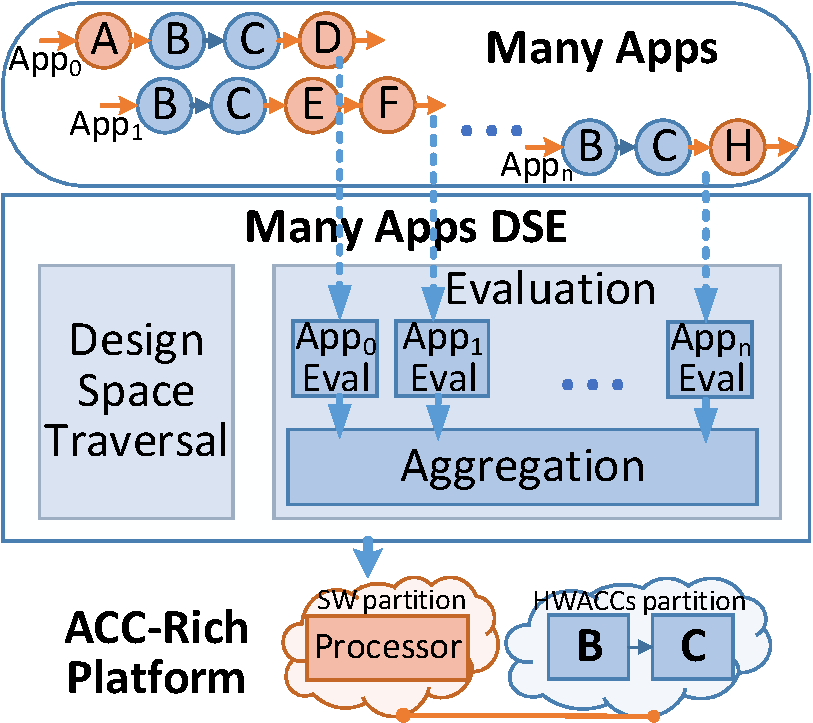
\includegraphics[width=.5\linewidth]{fig/MAARflow.pdf}
%	\caption{Promising Many Apps ACC-Rich Platform}
%	\label{fig:domainDSE}
%\end{figure}

%Tips: Mention Embedded or edge computing.

Using heterogeneous ACC-rich platforms~\cite{melpignano2012platform} that combine general-purpose processor(s) (SW) and custom ACCs (HW) is the primary approach for efficient, high-performance stream computing.
These platforms are typically designed targeting only a single application during allocation. Design Space Exploration (DSE) of one platform for each application is prohibitively expensive. In contrast to deep learning applications which often are computationally homogeneous and regular, such that a single monolithic accelerator can perform all linear algebraic computation required by deep learning algorithms, applications such as computer vision and software-defined radio demands a wide range of computationally intensive and functionality diverse heterogeneous accelerators (ACCs). The number of ACCs will increase dramatically, where individual ACCs are less monolithic but smaller and configurable. ACCs can be composed to accelerate larger kernels (or even applications).
%In contrast, platforms supporting many applications (e.g., FLP~\cite{tabkhi2016function}, Domain Platform~\cite{zhang2018ds}), that utilize similarities among applications, are promising to achieve flexibility to execute a set of applications efficiently.

\figref{fig:domainDSE} shows an example of a platform using $B$-$C$ ACCs to efficiently support many applications, which share $B$ and $C$ kernels. 
However, designing these platforms is a tremendous effort taking a vast amount of empiric knowledge into account. There is only little DSE methodology support for Many Applications ACC-Rich (MAAR) platforms because there is no existing evaluation to guide platform allocation for many applications. To feasibly allocate MAAR platforms, a MAAR DSE focusing on a set of applications, instead of individual applications in isolation, is needed.

\begin{figure}[ht]
  \centering
  \begin{minipage}[t]{0.24\textwidth}
    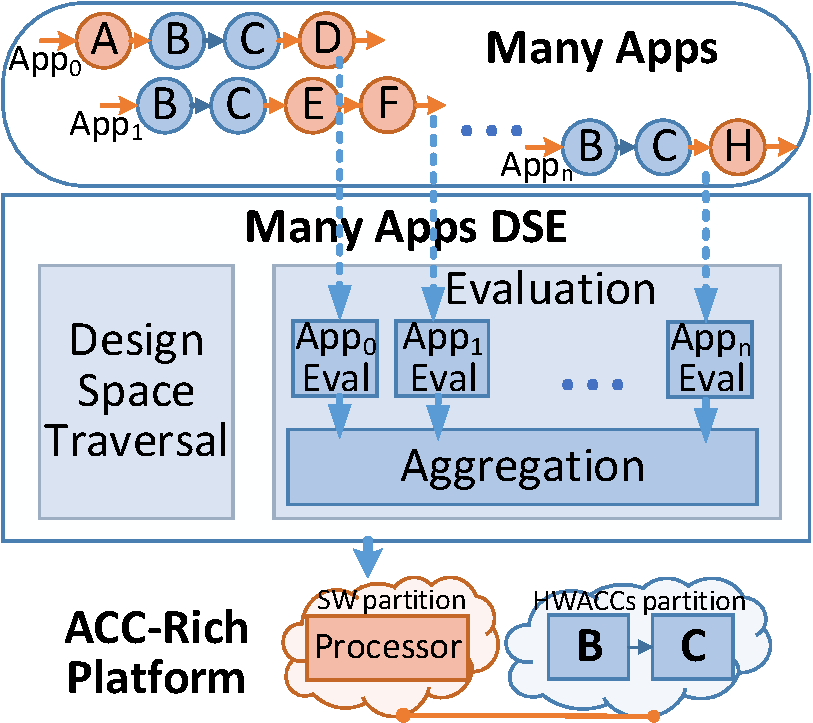
\includegraphics[width=.95\textwidth]{fig/MAARflow.pdf}
    \caption{Promising Many Apps ACC-Rich Platform}
    \label{fig:domainDSE}
  \end{minipage}%
  \hfill
  \begin{minipage}[t]{0.23\textwidth}
    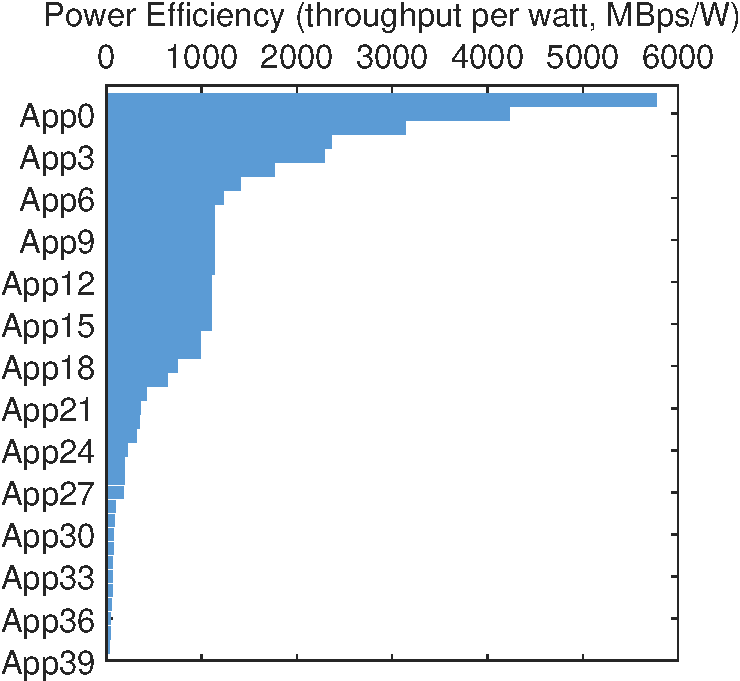
\includegraphics[width=1\textwidth]{fig/effIntro.pdf}
    \caption{Platform \newtext{Efficiency} for Applications}
	\label{fig:perf}
  \end{minipage}
\end{figure}

%\begin{figure}[h]
%	\centering
%	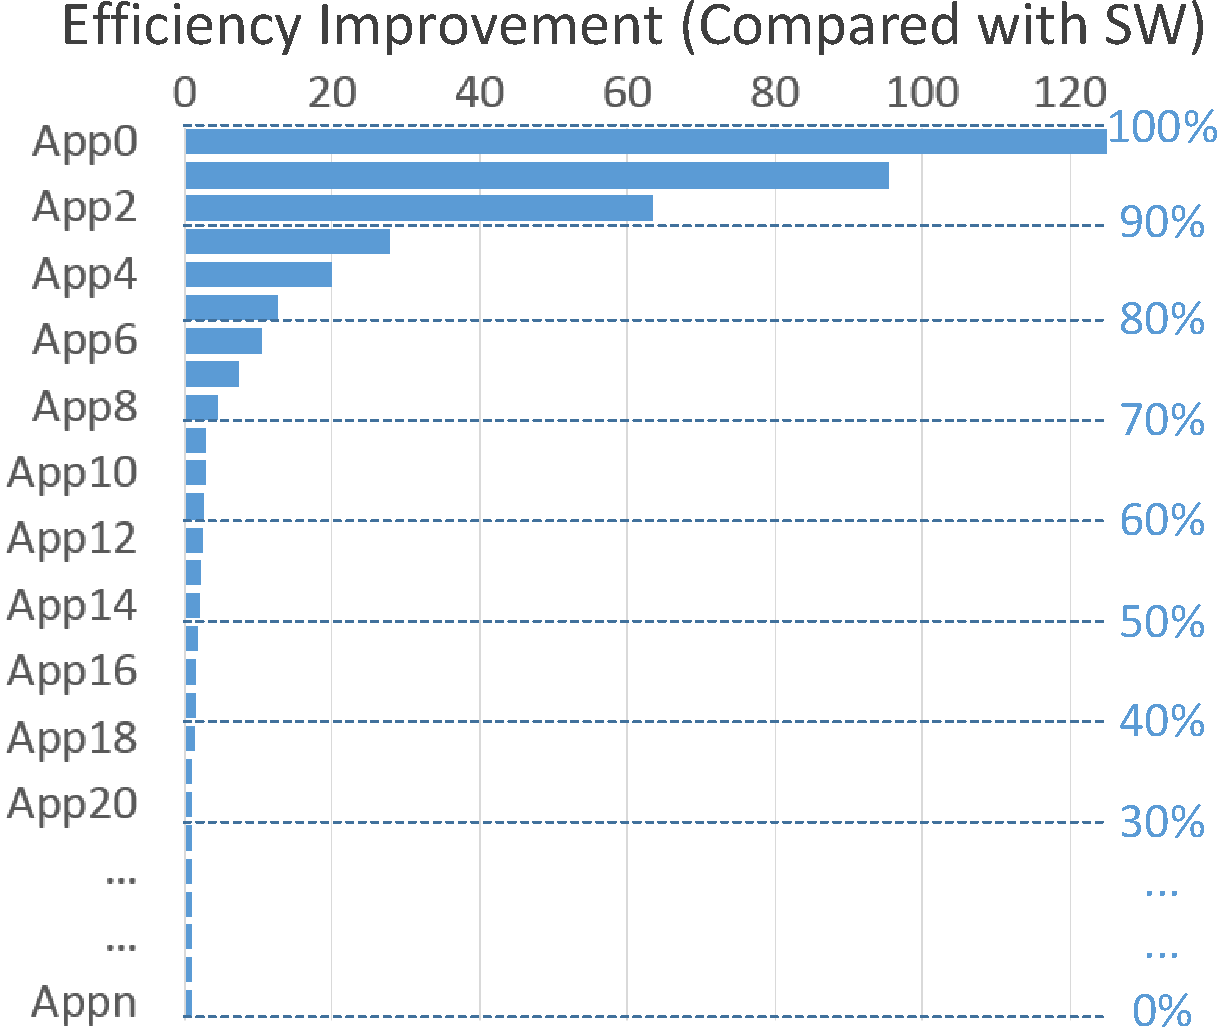
\includegraphics[width=.6\linewidth]{fig/Performance.pdf}
%	\caption{Domain Platform Efficiency Detail}
%	\label{fig:perf}
%\end{figure}

In \figref{fig:domainDSE}, many-application DSE has challenges in both design space traversal and a single design point (one platform) evaluation. Due to targeting to multiple applications, the design space of platform allocation is significantly larger than single application design, \newtext{and an efficient traversal is necessary.} 
Furthermore, the evaluation for many applications needs to have a fair focus on every application and provide an aggregated value to judge design quantitatively. Current platform evaluation primarily focuses the effects of the platform on one application in isolation. When moving to a set of applications, the simple average sum of all application performances is unfair. \figref{fig:perf} demonstrates the challenge of a MAAR platform evaluation. Because of the big variation among different applications' \newtext{efficiency} on the platform, the 10\% highest efficiency applications will dominate the DSE, if the evaluation simply sums all performances. As a result, the designed platform will not be efficient for many \newtext{low-efficiency} applications. To achieve a highly flexible and an efficient MAAR platform, a fair evaluation needs to aid the DSE in balancing the consideration of all applications.

%Hence, the traverse needs to be fast and efficient. 
%Besides high-speed request, 

%Unlike applications in a hand-composed benchmark, which balances contribution of each application to achieve a meaningful result, applications in a specified set of target applications have vastly different performances because of various parallelization and acceleration potential. 


This paper introduces MAAR DSE, guided by a platform evaluation for many applications with a balanced focus. To this end, the contributions of this paper are: (1) providing the flow of MAAR DSE, which is a combination of a heuristic traverse, elitist genetic algorithm (GA) and a fair evaluation for many applications; (2) defining relative efficiency of an application on a platform to have a normalized measure of improvement/achievement for different applications; (3) evaluating multiple methods to aggregate efficiency of many applications on a platform to quantitatively compare different platforms. The MAAR DSE fairly considers the contribution of many applications, and produces an efficient platform supporting all applications. In experiments using OpenVX applications, MAAR platforms achieve 3.09 times the average efficiency improvement of one application DSE (1appDSE), and 1.39 times the improvement of DSS, a previous domain platform DSE~\cite{zhang2018ds}. 
%With a budget of 12 ACCs, MAAR DSE's platform improves 67.5\% of applications by at least 3x, while 1appDSE only improves 15\% by 3x and DSS improves 42.5\% by 3x.

This paper is organized as follows: \secref{sec:related} summarizes the related works. \secref{sec:pre} introduces target ACC-rich platform and evaluation model for individual application. \secref{sec:eval} introduces MAAR DSE and fair MAAR platform evaluation methodology. \secref{sec:results} evaluates and analyzes the benefits of MAAR DSE with fair evaluation. Finally \secref{sec:conclusion} concludes this paper.


%\begin{figure}[h]
%    \centering
%    \begin{subfigure}[h]{.8\textwidth}
%        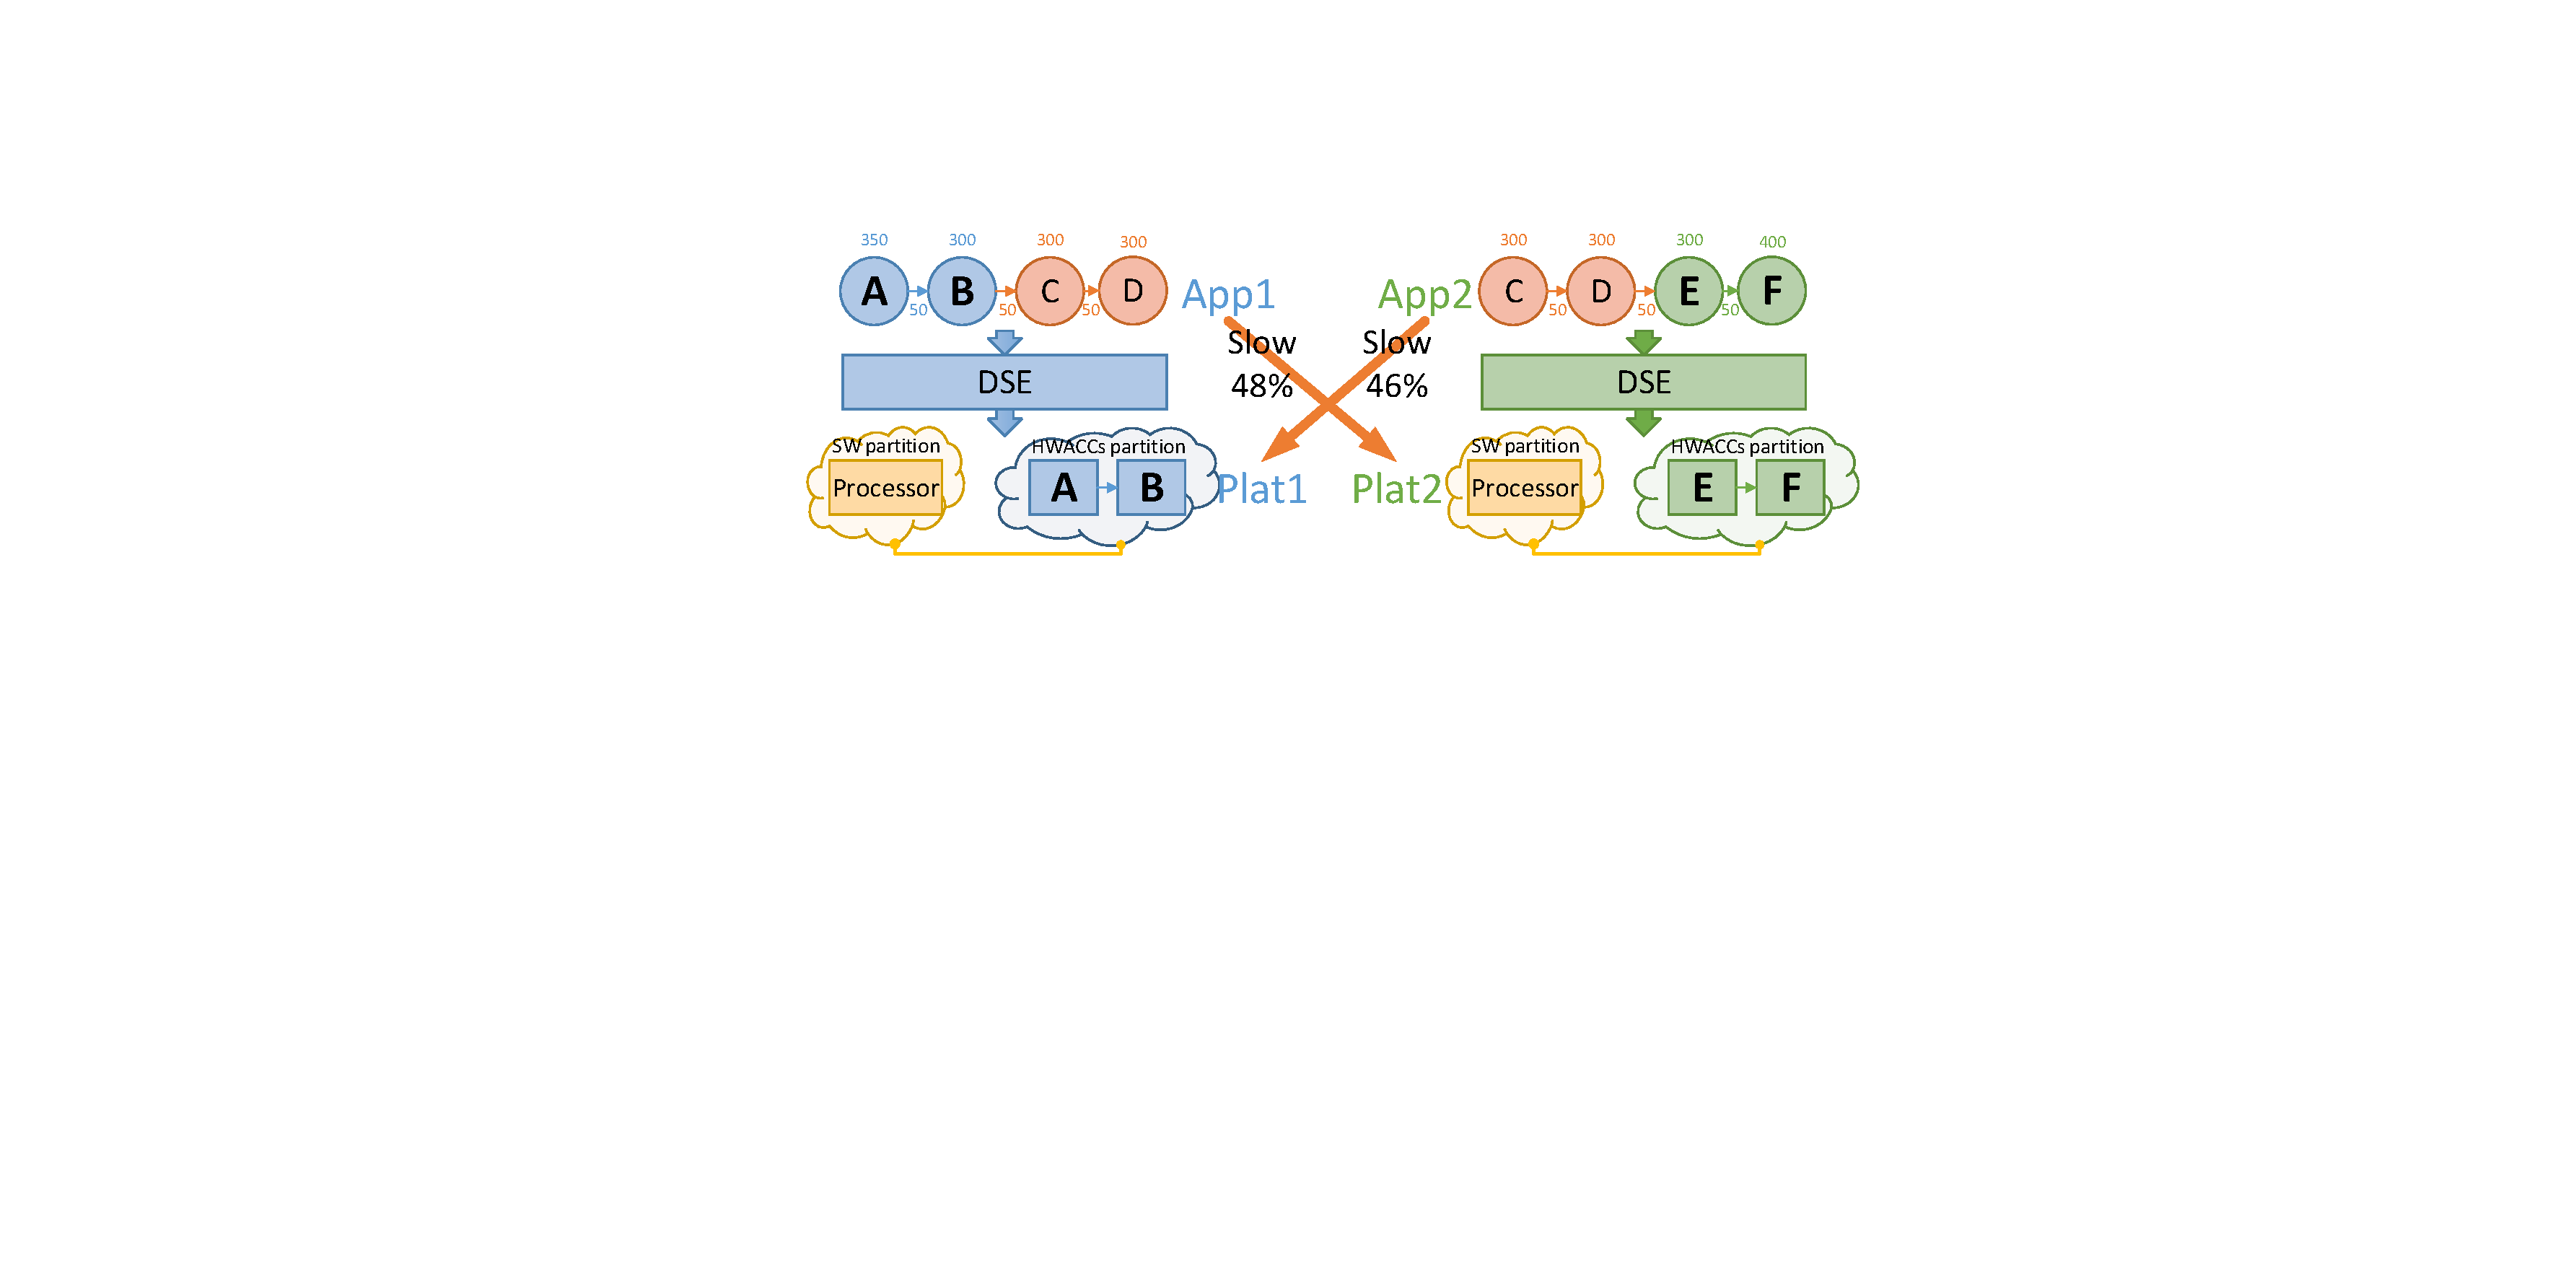
\includegraphics[h]{fig/pPlatApp.pdf}
%        \subcaption{App-Specific Platform]\label{fig:platApp}}
%    \end{subfigure}
%    \\
%    \begin{subfigure}[h]{.5\textwidth}
%        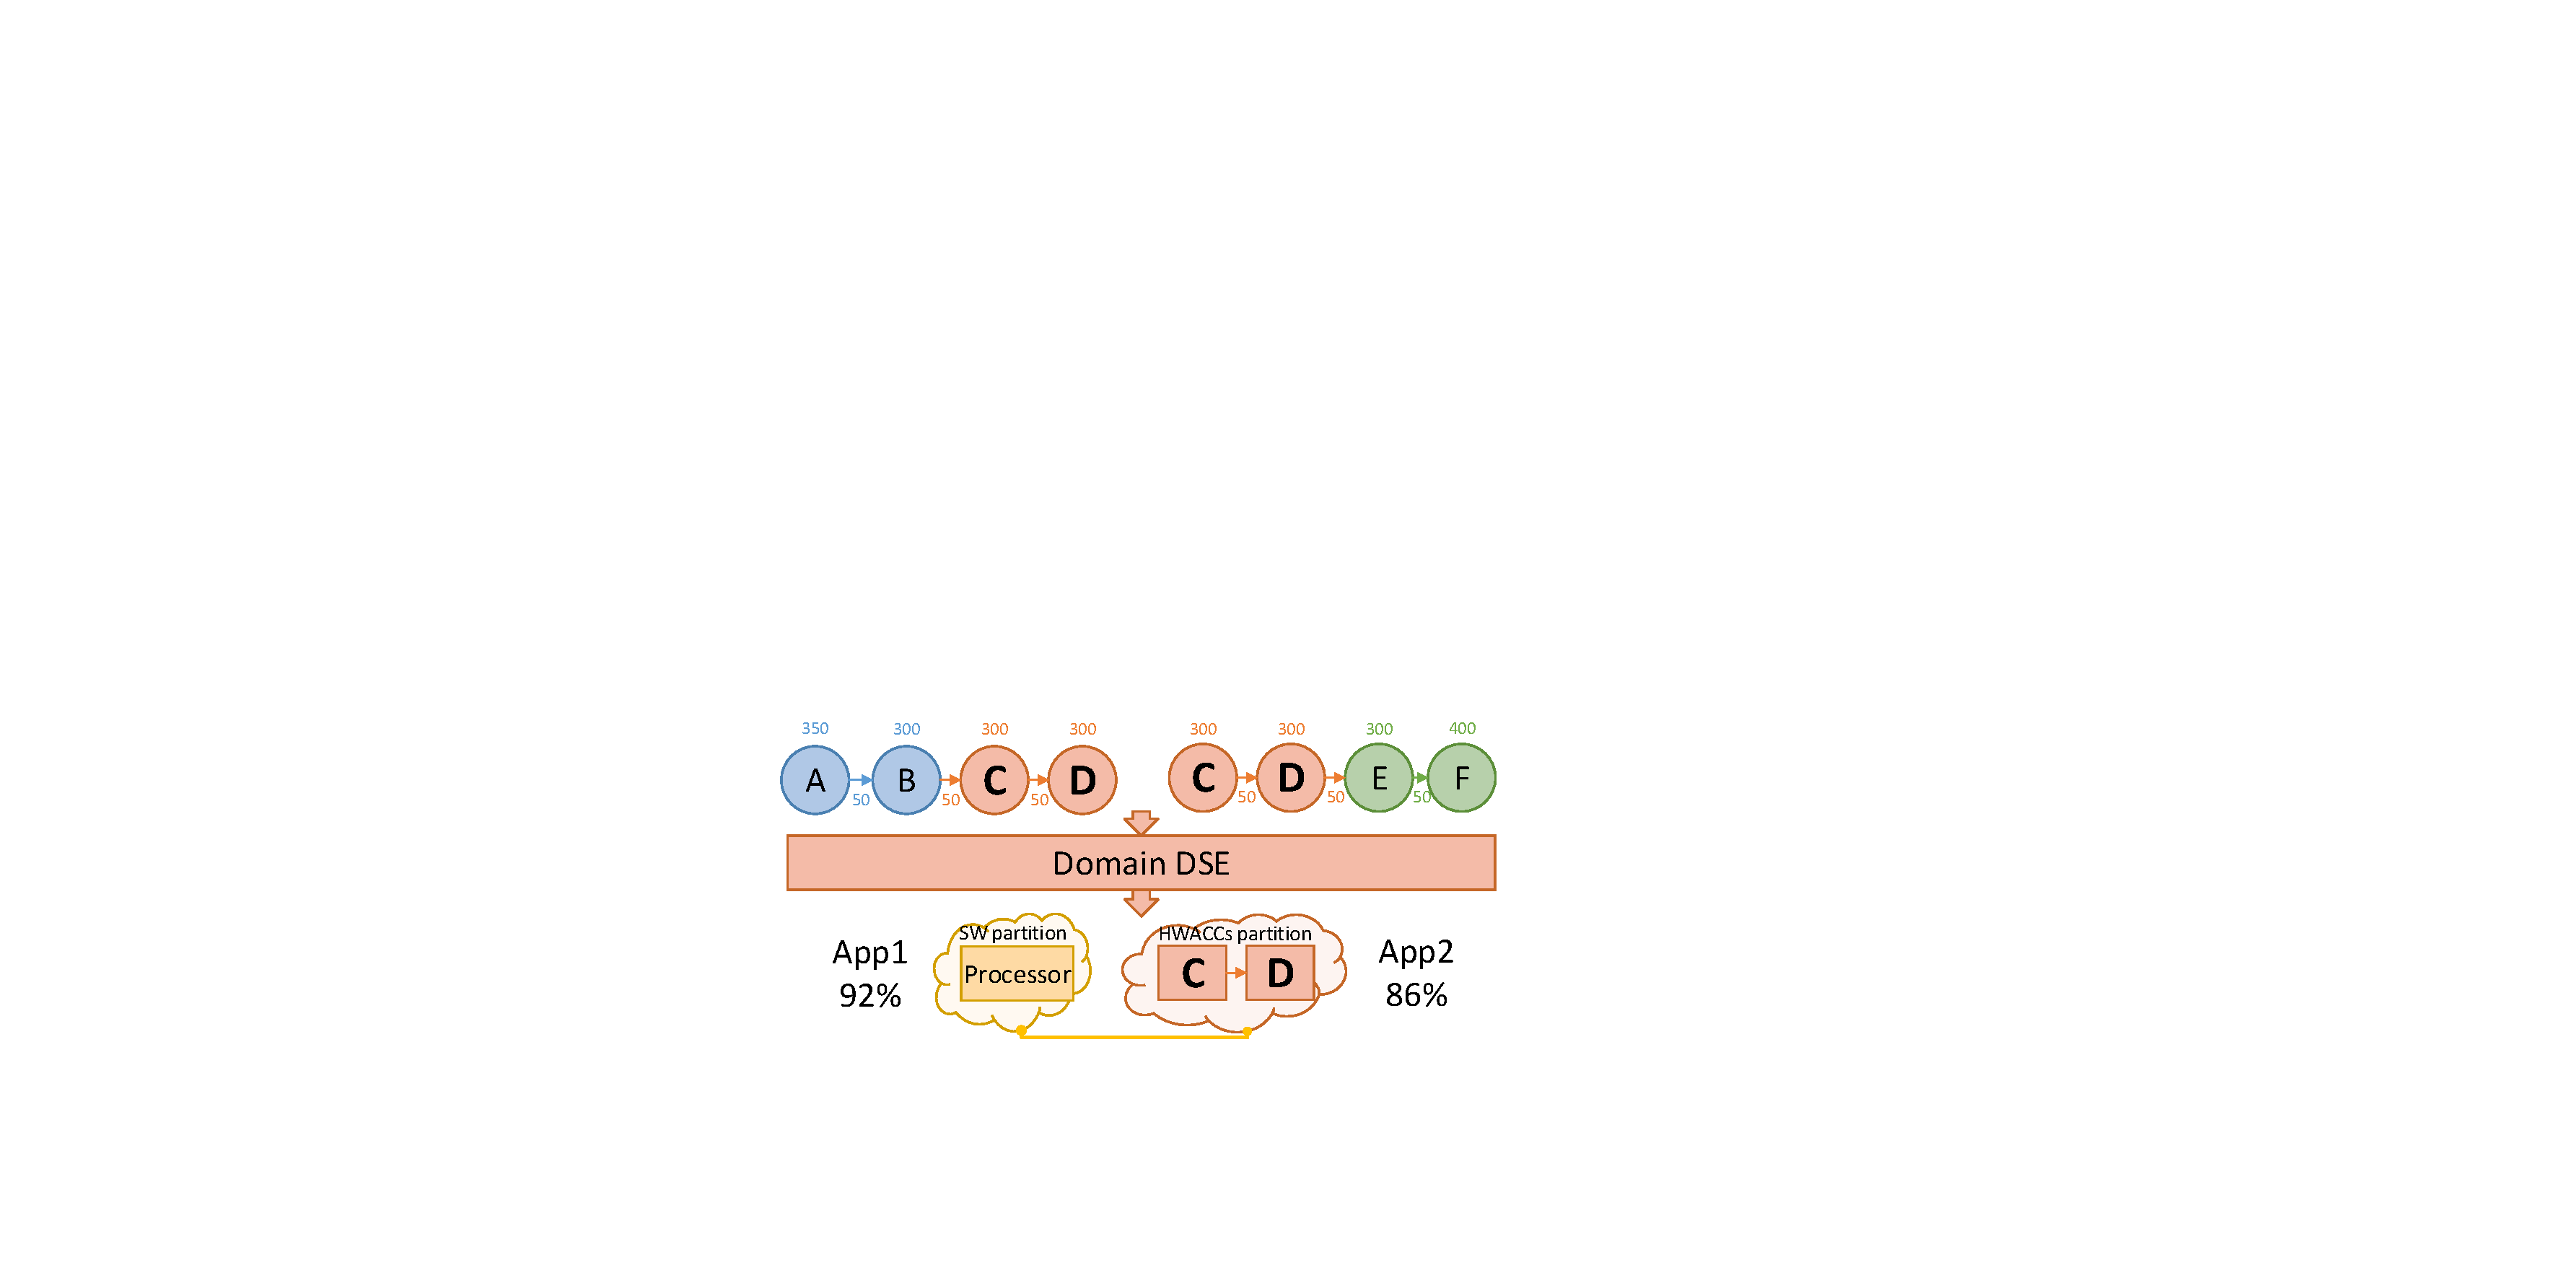
\includegraphics[h]{fig/pPlatDS.pdf}
%        \subcaption{Domain-Specific Platform]\label{fig:platDS}}
%    \end{subfigure}
%    \caption{Domain Platform: Penalty of Application Scope}
%    \label{fig:example}
%\end{figure}
\vspace{-2pt}
\section{Related Work}
\label{sec:related}

%Architecture
\newtext{
A larger number of architecture researches have been done for manually designing one common platform for homogeneous applications with repeated computation patterns, e.g. Minerva\cite{reagen2016minerva}, Eyeriss\cite{chen2018eyeriss} for Deep Neural Network applications with repeated convolution computing. 
To efficiently execute the application with heterogeneous kernels, monolithic ACC has been implemented at the beginning, e.g.\cite{tamitani1992encoder}\cite{chawla2016image}. 
However, the monolithic application-specific ACC has low flexibility and is not efficient for other applications. To support many applications in one architecture, ACC-rich platform\cite{cong2014accelerator}\cite{tabkhi2014function} is proposed, where many small ACCs can be composed to accelerate different large kernels (or even applications).
There are some other high-performance architecture works supporting many applications. 
Reconfigurable computing, such as \cite{wildermann2011operational}, aims to support multiple applications one at a time using FPGA, however, it relies on functional and structural similarities across reconfiguration cycles.
CPU associated with GPU\cite{grasso2014energy} is also a high-computing choice. However, GPU is too general and exceeds power and area limitation in embedded design\cite{maghazeh2013general}, especially in edge computing.
}

%Some promising architectures for many-application platforms have been proposed (e.g., \cite{tabkhi2014function, nowatzki2017domain}), but many-application DSE and platform evaluation have less been tackled. 

%Design Automation
\newtext{
Current design automation mainly focuses on one isolate application. The design flow covers two steps: platform architecture allocation and application-specific mapping (included binding and scheduling)\cite{SCE}\cite{Daedalus}\cite{gruttner2011challenges}.
There are huge researches about mapping different applications on the existing architecture\cite{marwedel2011mapping}\cite{quan2013scenario}. However, platform allocation for many applications is less touched. 
Some ideas about how to consider many applications can be extracted from platform-based design\cite{PBD}\cite{lukasiewycz2009combined}. It uses statistical information to design the platform template with fixed SW, partial network and memory hierarchy. Then application-specific resource allocation (e.g. ACC allocation) and mapping are applied\cite{PBDmapping}\cite{gladigau2010system}, which narrows the final architecture flexibility from many applications to a single application.
}


%algorithm
\newtext{In DSE algorithm. heuristic methods are widely used to deal with the vast and complex design space.}
The heuristics methods are comprised of an algorithm to explore design space and a fast evaluation/estimation to judge the performance of chosen platforms.
Some examples are genetic algorithms (GA)~\cite{quan2014towards}, simulated annealing~\cite{liang2013hardware}, tabu search~\cite{wu2013efficient}, and greedy algorithms~\cite{tang2015hardware}.
\newtext{These existing DSEs focus on allocating/mapping a platform for a single application because there is less existing platform evaluation that considers many applications.}
The only early example of a many-application DSE is Domain Score Selection (DSS)~\cite{zhang2018ds} which proposes a greedy approach for identifying similar function kernels for hardware acceleration, but it uses an unfair platform evaluation, comparing average throughput improvement, wherein a small number of high-performance applications dominate the evaluation. 

%Due to the vast and complex design space, heuristic methods are widely used in DSEs.
%The heuristics methods are comprised of an algorithm to explore design space and a fast evaluation/estimation to judge the performance of chosen platforms.
%Some examples are genetic algorithms (GA)~\cite{quan2014towards}, simulated annealing~\cite{liang2013hardware}, tabu search~\cite{wu2013efficient}, and greedy algorithms~\cite{tang2015hardware}.
%These existing DSEs focus on allocating a platform for a single application, because there is less existing platform evaluation that considers many applications. 

%Some ideas about how to consider many applications can be extracted from platform-based computing which uses statistical information to design the platform template and application-specific mappings~\cite{graf2014multi, gladigau2010system}. However, more specialization for a wider set of applications is needed. Reconfigurable computing, such as \cite{wildermann2011operational}, aims to support multiple applications one at a time, however, it relies on functional and structural similarities across reconfiguration cycles.

%Some promising architectures for many-application platforms have been proposed (e.g., \cite{tabkhi2014function, nowatzki2017domain}), but many-application DSE and platform evaluation have not yet been tackled. 
%An early example of a many-application DSE is Domain Score Selection (DSS)~\cite{zhang2018ds} which proposes a greedy approach for identifying similar function kernels for hardware acceleration, but it uses an unfair platform evaluation, comparing average throughput improvement, wherein a small number of high-performance applications dominate the evaluation. 
\vspace{-2pt}
\section{Preliminaries}
\label{sec:pre}

To set the stage of our proposed MAAR platform evaluation and DSE, this section introduces the target platform and the evaluation method for a single application on a platform.


%\vspace{-4pt}
\subsection{Target Platform}

ACC-rich platforms include hardware accelerators (ACCs) and programmable processors (CPU, GPU, DSP). \figref{fig:plat} illustrates the target platform for the context of this work. A streaming application $A, B, C, D$ is mapped across SW and HW. Each ACC has a dedicated \newtext{Scratch Pad Memory (SPM)}. All ACCs are aggregated to a HW partition with a shared SPM across all ACCs. ACCs can communicate with each other, and their communication traffic is hidden from system communication fabric (e.g., $B$, $C$). For simplicity, we assume direct n:n communication within the HW partition. Conversely, ACCs and SW kernels communicate through the system streaming fabric (e.g., $A$ to $B$, and $C$ to $D$) which results in throughput penalties.

\vspace{-2pt}
\begin{figure}[h]
	\centering
	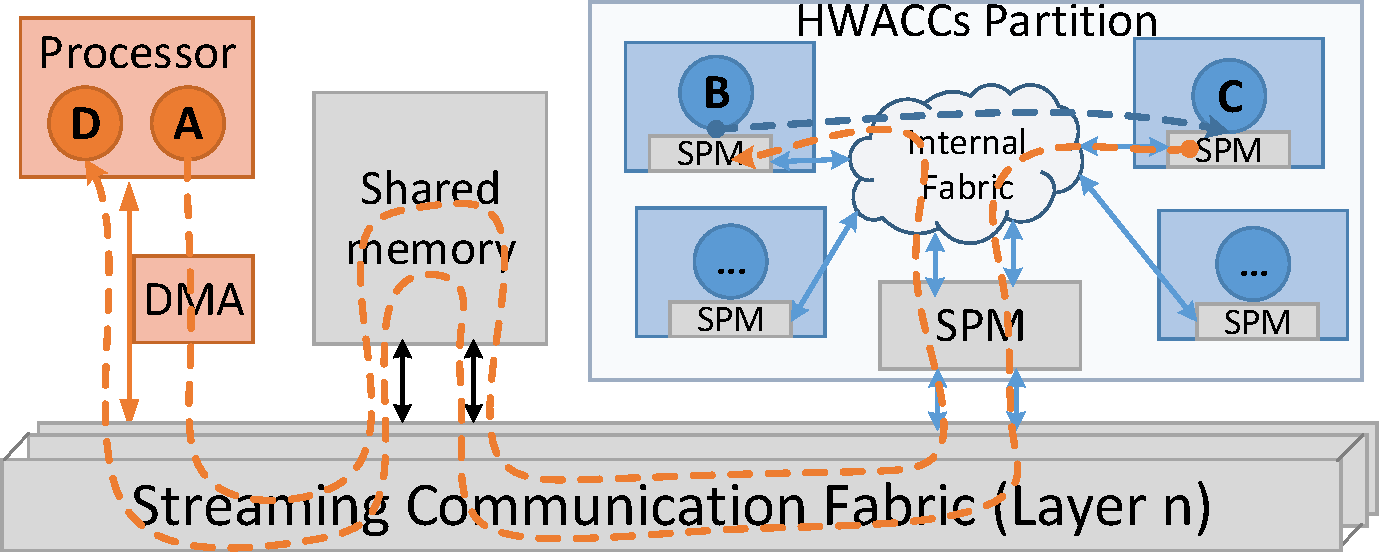
\includegraphics[width=.8\linewidth]{fig/pPlat.pdf}
	\vspace{-4pt}
	\caption{Target Platform}
	\label{fig:plat}
\end{figure}


\vspace{-2pt}
\subsection{Analytic Evaluation}
\label{subsec:ana}

Evaluating an individual application on a platform follows a speed/accuracy trade-off.
The evaluation request in many-application platform design is vast due to (a) the enormous domain design space which needs to be traversed (b) the number of applications which must be evaluated for each allocation. 
An abstract and dramatically fast evaluation, analytic evaluation, is desired to evaluate many more points at the cost of accuracy.

%\begin{figure}[h]
%	\centering
%	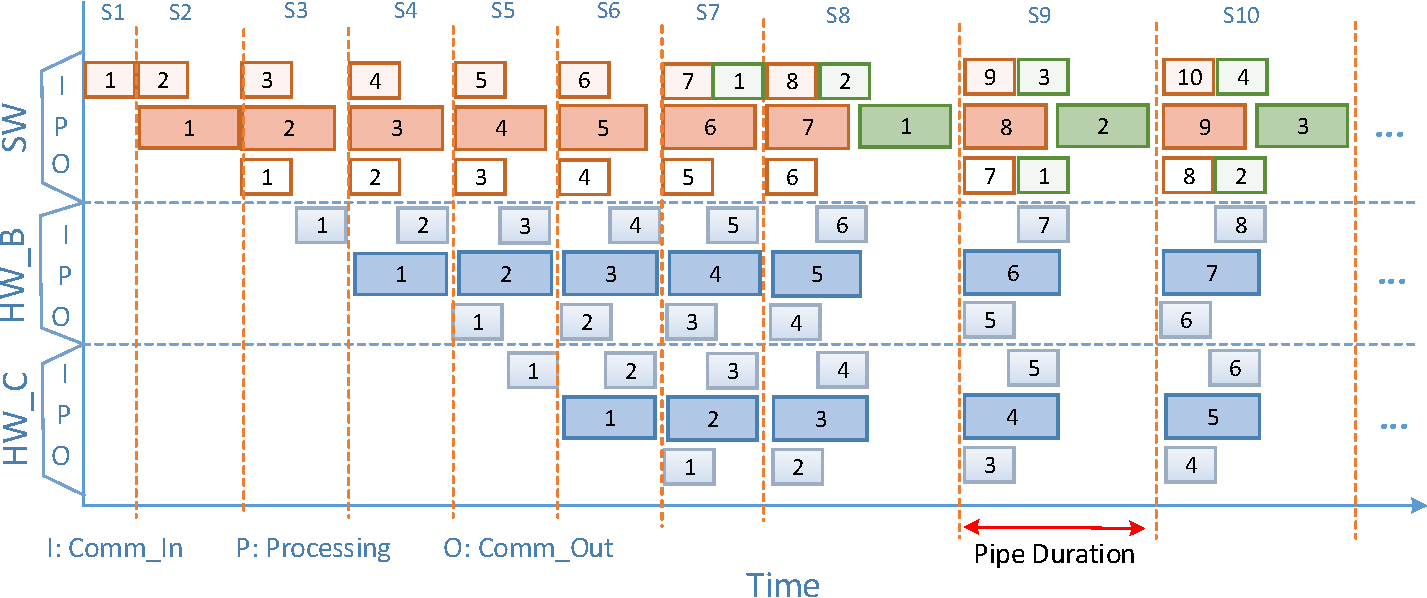
\includegraphics[width=\linewidth]{fig/pPipe.pdf}
%	\caption{Timing diagram of Architecture}
%	\label{fig:Pipe}
%\end{figure}

In analytic evaluation~\cite{Teimouri_TCAD_2018}, the kernels in a streaming application operate as producers and consumers of the streaming data and form a pipeline. 
%\figref{fig:Pipe} visualizes the pipeline execution for two ACCs and one SW core. 
Each pipe stage overlaps communication (in/out) with processing due to double buffering. Actors execute concurrently given their dependencies across different processing components. Actors mapped to the same component execute sequentially.
Our Analytic Evaluation model computes the throughput ($Th$), latency ($L$) and energy consumption ($EC$) of an application based on the inter-kernel pipelined execution.
\newtext{Compared with virtual platforms evaluation generated by the System-on-Chip Environment (SCE) \cite{SCE}, the performance fidelity of Analytic Evaluation is 98\%.}


\vspace{-2pt}
\section{Unified Platform Allocation}
\label{sec:eval}

This section introduces Unified Platform Allocation (UPA) supporting many applications. \secref{subsec:MAAR} introduces a heuristic method, an elitist genetic algorithm, to efficiently traverse the large design space. To achieve fair evaluation for many applications, \secref{subsec:relativeEff} defines relative efficiency which balances across many vastly different applications, and \secref{subsec:aggregation} proposes and evaluates different methods to fairly aggregate efficiency across many applications to evaluate different platforms.

\newcommand{\dsename}[1]{\textit{#1}}

\vspace{-2pt}
\subsection{UPA Flow and Traversal}
\label{subsec:MAAR}

Novel allocation approaches are needed that broaden the design scope from single application to a set of applications in order to design a unified platform. The enormous design space renders exhaustive search unfeasible, requiring heuristics for sparse sampling. UPA employs an elitist Genetic Algorithm (GA)~\cite{quan2014towards} to support efficient design space traversal.

%\vspace{-4pt}
\begin{figure}[h]
	\centering
	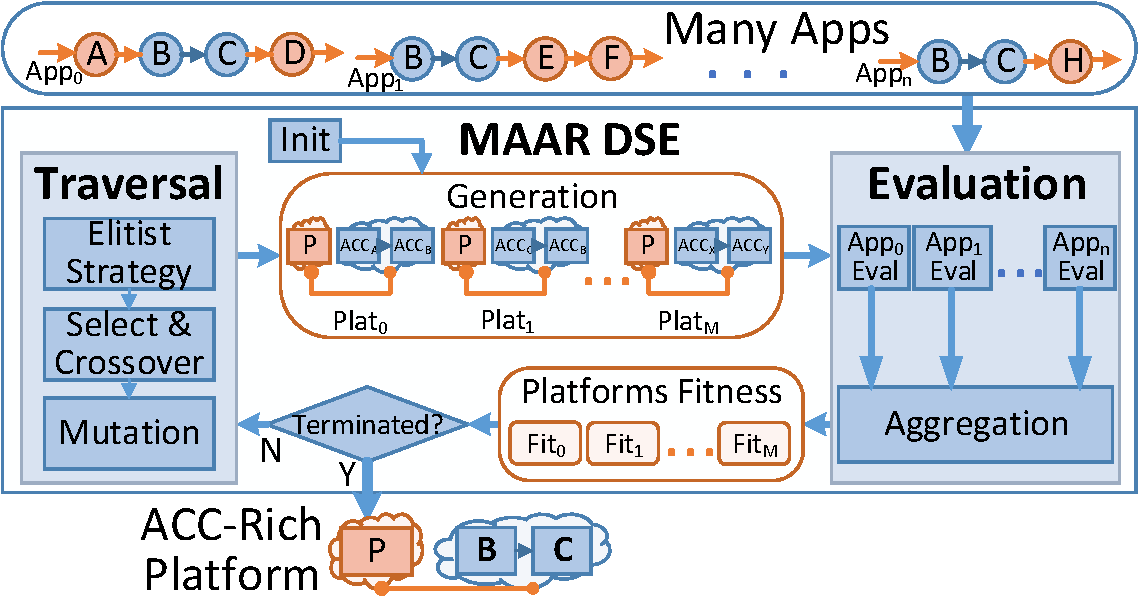
\includegraphics[width=.9\linewidth]{fig/MAARflowDetial.pdf}
	\vspace{-4pt}
	\caption{UPA Detial Flow}
	\label{fig:MAARflowDetial}
\end{figure}

\figref{fig:MAARflowDetial} overviews UPA flow. The generation configuration is captured in a set of chromosomes, representing platforms. Each chromosome captures platform allocation of kernels across many applications as a set of genes. After randomly generating an initial generation, the UPA \dsename{Evaluation} analyzes the fitness of each chromosome/platform. In \dsename{Traverse}, the \dsename{Elitist Strategy} tracks global top 10\% platforms (across all generations). It replaces the bottom 10\% each generation with the global top 10\%. From this, \dsename{Selection \& Crossover} selects pairs of promising chromosomes with roulette wheel selection according to their fitness and swaps genes among them. To further speed up exploration, \dsename{Mutation} employs a local search method guided by analytic evaluation to propagate the best neighbor of the design point. The resulting generation is evaluated and the process repeats until the \dsename{Termination} condition (no better platform for 10 iterations) is reached.
\vspace{-2pt}
\subsection{Balancing Across Vastly Different Apps}
\label{subsec:relativeEff}

Platform evaluation is key to UPA. Evaluating many applications poses two challenges: (a) balancing performance for vastly different applications, and (b) fair aggregation of performances across all applications. This section introduces relative efficiency as a measure of performance across applications. \secref{subsec:aggregation} discusses the aggregation.

Platform design can optimize various goals, e.g., minimize energy consumption or maximize throughput, under various constraints (e.g., cost, area). In this work, we focus on maximizing energy efficiency, which combines performance and energy as a goal, with area (in number of ACCs) as a constraint. Eq.~\eqref{eq:pipe} calculates the energy efficiency ($EFF$) of the platform using the analytic model in \secref{subsec:ana}. In streaming, energy efficiency can be expressed as throughput [bytes/second] per watt of power~\cite{zhou2013energy}. Throughput is equal to output volume per iteration $D_{out}$ over the latency time $L$. The power is equal to energy consumption $EC$ over its latency $L$.

\vspace{-8pt}
\begin{equation}
	EFF = \left. \frac{Th}{Power} \right\vert\ Th = \frac{D_{out}}{L},\ Power = \frac{EC}{L}
\label{eq:pipe}
\end{equation}

However, energy efficiency differs vastly across applications, since applications have differing potentials for efficiency. Hence, direct comparison or aggregation is not suitable. To fairly judge platform efficiency across applications, it needs to be normalized to some measure of an application's potential for efficiency.

Efficiency improvement is normalized to the efficiency of running in software (SW) (application's efficiency lower bound), and efficiency achievement is normalized to running on an Own Optimal Dedicated Platform (ODP) (upper bound). Given a ACC budget, each application has its own optimal platform, obtained through one application exploration, e.g. exhaustive search. As a result, an ODP is the efficiency upper boundary for its application but is not designed for other applications.

Using the two normalizations, Eq.~\eqref{eq:rel} defines two relative efficiencies balancing across applications. $rEFF_{SW}$ represents the energy efficiency improvement of an application $a_i$ on platform $p_X$ over $SW$, and $rEFF_{ODP}$ represents the achievement of $a_i$ on $p_X$ relative to $ODP$.

\vspace{-8pt}
\begin{equation}
\begin{split}
	rEFF_{SW}(a_{i}, p_{X}) &= EFF(a_{i}, p_{X}) / EFF(a_{i}, p_{SW}) \\
	rEFF_{ODP}(a_{i}, p_{X}) &= EFF(a_{i}, p_{X}) / EFF(a_{i}, p_{ODP})
\label{eq:rel}
\end{split}
\end{equation}

For illustration, \figref{fig:eff} plots the relative efficiency of 40 OpenVX applications on one Unified Platform (UP, blue) with 10 ACCs. While the normalizations help reduce variations in efficiency, they don't eliminate all of the variation due to applications' potentials for efficiency. This poses a challenge for aggregation to evaluate a platform, since it should not over-represent high-efficiency applications.

\vspace{-4pt}
\begin{figure}[h]
	\centering
		\subfloat[Efficiency Improvement]{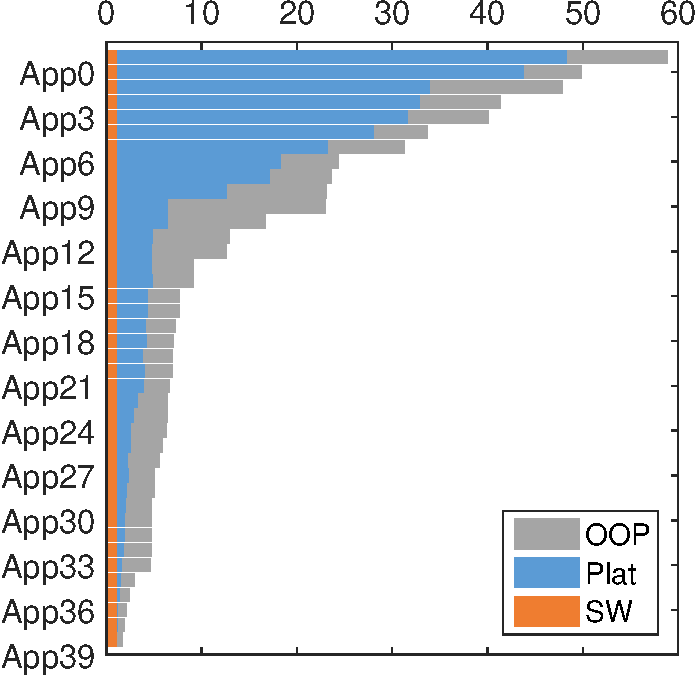
\includegraphics[width=.46\linewidth]{fig/effSW.pdf}\label{fig:effSW}}
		\hfill
		\subfloat[Efficiency Achievement]{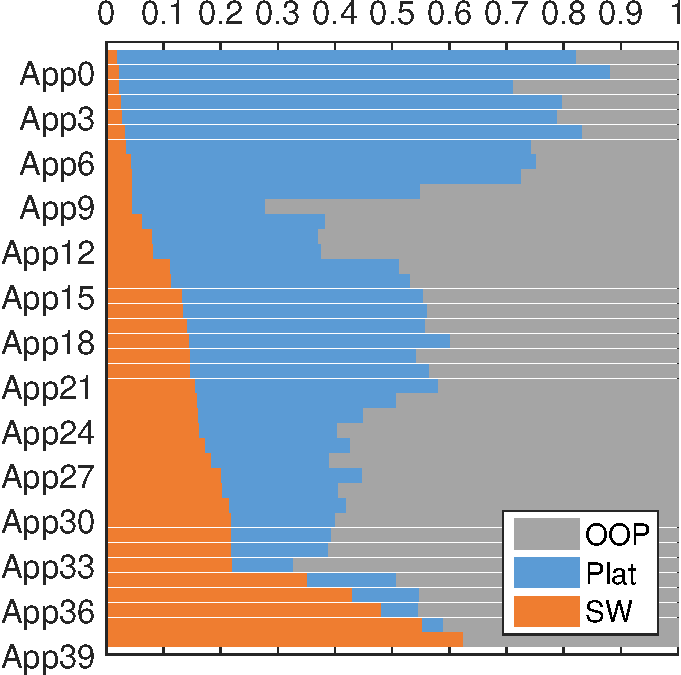
\includegraphics[width=.45\linewidth]{fig/effOOP.pdf}\label{fig:effOOP}}
    \vspace{-8pt}
	\caption{Relative Efficiency}
	\label{fig:eff}
\end{figure}
\vspace{-2pt}
\subsection{Fair Aggregation across Many Apps}
\label{subsec:aggregation}

In order to quantitatively reason about platforms, the normalized application efficiencies need to be aggregated into a single fitness value. This section proposes and compares aggregation options.

Illustrating the aggregation challenge, \figref{fig:eff} shows normalized efficiencies of application on an example Unified Platform (UP, blue) normalized by the lower bound SW platform (orange) in \figref{fig:effSW} and by the upper bound ODP (grey) in \figref{fig:effOOP}. In \figref{fig:effSW}, the relative efficiency of SW is always equal to 1, because it is normalized by itself. The ODP has higher $rEFF_{SW}$ than the UP for each application because ODP is the optimal platform design for each application. \figref{fig:effOOP} shows relative efficiency compared with ODP $rEFF_{ODP}$ for SW, UP and ODP. Similarly, ODP always has a $rEFF_{ODP}$ of 1 because it is normalized by itself. UP has $rEFF_{ODP}$ between SW and ODP, because UP accelerates some kernels to achieve better performance than SW, and is not the application own optimal platform, so it performs worse than the ODP.

\subsubsection{Average Aggregation}

To judge the fitness of a platform for all applications, the intuitive method is to aggregate the overall efficiency increase or loss across all applications.
In \figref{fig:effSW}, a MAAR platform with a more blue area (or a less grey area) is better, because it has a more overall increase (or a less loss). 
To achieve the best MAAR platform $p_{X}$, DSE should maximize the blue area ($Area_{b}$) or minimize the grey area ($Area_{g}$). 
Assuming the length of total number of applications in y-axis is equal to 1, 
$Area_{b}$ is equal to $\sum_{i=0}^{\#a} ( rEFF_{SW}(a_{i}, p_{X}) -  rEFF_{SW}(a_{i}, p_{SW}) ) / \#a $, and $Area_{g}$ is $\sum_{i=0}^{\#a} ( rEFF_{SW}(a_{i}, p_{OOP}) -  rEFF_{SW}(a_{i}, p_{X}) ) / \#a $.
After simplification, both maximizing $Area_b$ and minimizing $Area_g$ become equivalent to maximizing $\sum_{i=0}^{\#a} rEFF_{SW}(a_{i}, p_{X}) / \#a$, which is the average efficiency improvement of platform $p_{X}$.  

Both methods are equivalent because of the SW and OOP platforms are fixed for a set of applications, so the summed SW and OOP efficiency areas are constant. 
Therefore, maximizing the efficiency difference between platform $p_{X}$ and SW, or minimizing the difference between $p_{X}$ and OOP leads to the same result, which is to maximize the average efficiency improvement of $p_{X}$. 
The average of $rEEF_{SW}$ ($A \mhyphen SW$) across all applications becomes the first MAAR DSE fitness function, which is represented in the first line of Eq.~\eqref{eq:avg}.

\vspace{-8pt}
\begin{equation}
\begin{split}
	A\mhyphen SW (p_{X}) &= \sum_{i=0}^{\#a} rEFF_{SW}(a_{i}, p_{X}) / \#a \\
	A\mhyphen OOP (p_{X}) &= \sum_{i=0}^{\#a} rEFF_{OOP}(a_{i}, p_{X}) / \#a
\label{eq:avg}
\end{split}
\end{equation}

Similarly in \figref{fig:effOOP}, maximizing the difference in $rEFF_{OOP}$ between MAAR platform $p_{X}$ and SW, and minimizing the difference between $p_{X}$ and OOP are both equivalent to maximize the average efficiency achievement $rEFF_{OOP}$, as displayed in the second line of Eq.~\eqref{eq:avg}. $A \mhyphen OOP$ is the second proposed fitness function.
\subsubsection{Median Aggregation}

Instead of focusing on the overall relative efficiency of all applications, maximizing the median efficiency across applications is another fitness function choice. 
Because median-maximizing behavior is more resilient to outliers, it is a good candidate to balance acceleration potential across many applications, and the median-maximizing guided allocation may provide a more balanced platform with a good efficiency distribution of applications. 
Eq.~\eqref{eq:med} shows two median maximizing fitness functions of two relative efficiencies $rEFF_{SW}$ and $rEFF_{ODP}$. 

\vspace{-4pt}
\begin{equation}
\begin{split}
	M\mhyphen SW (p_{X}) &= med(rEFF_{SW}(a_{i}, p_{X})),   i = 0,1,...,\#a \\
	M\mhyphen ODP (p_{X}) &= med(rEFF_{ODP}(a_{i}, p_{X})), i = 0,1,...,\#a
\label{eq:med}
\end{split}
\end{equation}
\subsubsection{Log Area Aggregation}

In previous average aggregation, high relative efficiency applications have more effect on fitness. The value difference between high and low relative efficiency across applications is still a little significant, especially in $rEFF_{SW}$. To shrink the difference among applications and pay more attention to low-efficiency applications, a new aggregation with logarithm is proposed.
Instead of maximizing/minimizing the relative efficiency difference between UP and SW/ODP, the new method ($Alog$) first takes the logarithm of the efficiency to shrink the difference in relative efficiency among applications, then maximizes/minimizes the resulting logarithmic area.

\begingroup\makeatletter\def\f@size{6.9}\check@mathfonts
\vspace{-8pt}
\begin{equation}
\begin{split}
	Alog\mhyphen SW(p_{X})
	&= \sum_{i=0}^{\#a} ( \log rEFF_{SW}(a_{i}, p_{X}) - \log rEFF_{SW}(a_{i}, p_{SW}) ) / \#a \\
	&= \sum_{i=0}^{\#a} ( \log rEFF_{SW}(a_{i}, p_{X}) ) / \#a 
	%&= \sum_{i=0}^{\#a} ( \log EFF(a_{i}, p_{X}) - \log EFF(a_{i}, p_{SW}) - \log 1 ) / \#a \\
	%&= \sum_{i=0}^{\#a} ( \log EFF(a_{i}, p_{X}) ) / \#a - \sum_{i=0}^{\#a} ( \log EFF(a_i, p_{SW}) ) / \#a
\label{eq:logSW}
\end{split}
\end{equation}
\endgroup

\begingroup\makeatletter\def\f@size{6.9}\check@mathfonts
\vspace{-8pt}
\begin{equation}
\begin{split}
	Alog\mhyphen ODP(p_{X})
	&= \sum_{i=0}^{\#a} ( \log rEFF_{ODP}(a_{i}, p_{X}) - \log rEFF_{ODP}(a_{i}, p_{SW}) ) / \#a \\
	&= \sum_{i=0}^{\#a} ( \log \frac{EFF(a_{i}, p_{X})}{EFF(a_{i}, p_{ODP})} - \log \frac{EFF(a_{i}, p_{SW})}{EFF(a_{i}, p_{ODP})} ) / \#a \\
	&= \sum_{i=0}^{\#a} ( \log rEFF_{SW}(a_{i}, p_{X}) ) / \#a
	%&= \sum_{i=0}^{\#a} ( \log EFF(a_{i}, p_{X}) ) / \#a - \sum_{i=0}^{\#a} ( \log EFF(a_i, p_{SW}) ) / \#a
\label{eq:logOOP}
\end{split}
\end{equation}
\endgroup


Eq.~\eqref{eq:logSW} shows the the log area of the efficiency improvement $Alog\mhyphen SW$. 
Since $\log rEFF_{SW}(a_i, p_{SW}) = 0$ for all $a_i$, $Alog\mhyphen SW$ becomes maximizing $\sum_{i=0}^{\#a} \log rEFF_{SW}(a_{i}, p_{X}) / \#a$. In Eq.~\eqref{eq:logOOP}, the log area of achievement $Alog\mhyphen ODP$ becomes the same as $Alog\mhyphen SW$, after relative efficiency transformation and logarithm simplification.


\begingroup\makeatletter\def\f@size{6.9}\check@mathfonts
\vspace{-8pt}
\begin{equation}
\begin{split}
	Alog(p_{X}) &\equiv Alog\mhyphen SW(p_{X}) \equiv Alog\mhyphen ODP(p_{X}) \\
	&= \sum_{i=0}^{\#a} ( \log rEFF_{SW}(a_{i}, p_{X}) ) / \#a  \\
	&= \sum_{i=0}^{\#a} ( \log \frac{EFF(a_{i}, p_{X})}{EFF(a_{i}, p_{SW})}) / \#a \\
	&= \sum_{i=0}^{\#a} ( \log EFF(a_{i}, p_{X}) ) / \#a - \sum_{i=0}^{\#a} ( \log EFF(a_i, p_{SW}) ) / \#a
\label{eq:logDetial}
\end{split}
\end{equation}
\endgroup


Next in Eq.~\eqref{eq:logDetial}, $Alog$ can be transformed into two components, the logarithmic area of platform $p_{X}$ efficiency subtracts the logarithmic area of software efficiency. 
Since the efficiency of an application in software $EFF(a_i, p_{SW})$ is constant for all applications, it does not affect which platform $Alog\mhyphen SW$ is maximized for. Therefore, the normalization factor becomes unimportant in log area, so $Alog$ becomes equivalent to the log area of efficiency as shown in Eq.~\eqref{eq:log}. The fact that the normalization factor ``disapears'' in $Alog$ suggests that taking the logarithm of the efficiency of an application removes its dependence on the application's potential for efficiency without the need for a specific normalization.


\begingroup\makeatletter\def\f@size{6.9}\check@mathfonts
\vspace{-8pt}
\begin{equation}
\begin{split}
	Alog(p_{X}) = \sum_{i=0}^{\#a} ( \log EFF(a_{i}, p_{X}) ) / \#a	
\end{split}
\label{eq:log}
\end{equation}
\endgroup

\tabref{tab:fit} summarizes all proposed aggregation methods, which decide the fitness functions (evaluation) in UPA. There are two average aggregation methods using $rEFF_{SW}$ and $rEFF_{ODP}$, two median aggregation methods also using $rEFF_{SW}$ and $rEFF_{ODP}$, and one logarithmic area aggregation method. 


\begin{table}[h]
	\caption{Fitness Functions (Evaluations) in UPA}
	\vspace{-8pt}
	\label{tab:fit}
	\centering
	\begin{tabular}{p{0.10\linewidth}|p{0.35\linewidth}|p{0.35\linewidth}}
		\toprule
		& $rEFF_{SW}$ & $rEFF_{ODP}$ \\
		\midrule
		\hline
		Avg (A-)& \(\displaystyle \sum_{i=0}^{\#a} rEFF_{SW}(a_{i}, p_{X})/\#a \) & \(\displaystyle\sum_{i=0}^{\#a} rEFF_{ODP}(a_{i}, p_{X})/\#a \)\\
		\hline
		%\multirow{2}{*}{Median (M-)} & \(\displaystyle med(rEFF_{SW}(a_{i}, p_{X})) \),  &	\(\displaystyle med(rEFF_{OOP}(a_{i}, p_{X})) \), \\
		%& $i = 0,1,...,\#a$ & $i = 0,1,...,\#a$ \\
		
		Median (M-) & \(\displaystyle med(rEFF_{SW}(a_{i}, p_{X})) \),  $i = 0,1,...,\#a$  &	\(\displaystyle med(rEFF_{ODP}(a_{i}, p_{X})) \),  $i = 0,1,...,\#a$ \\
		
		\hline
		logArea (Alog)& \multicolumn{2}{c}{\(\displaystyle \sum_{i=0}^{\#a} ( \log (EFF(a_{i}, p_{X})) ) / \#a \)}\\
		\bottomrule
	\end{tabular}
\end{table}

   

























\vspace{-2pt}
\section{Experimental Results}
\label{sec:results}


This section evaluates the benefit of executing many applications on a UPA platform. 
After defining the experimental setup in \secref{subsec:res-setup}, \secref{subsec:res-overall} first compares with other platform allocations. \secref{subsec:res-agg} will then gives insights on evaluating different aggregations in UPA evaluation. 


%\vspace{-2pt}
\subsection{Experiment Setup}
\label{subsec:res-setup}

In the analytic evaluation, the target unified platform settings \newtext{are: (1) An ARM CortexA57 processor with} 4 ARMv8-A cores simulated at the 1.4GHz clock frequency, analytic computing performance of each core is 2000 MIPS. (2) A multi-layer AMBA AHB (32 bit-width, 200MHz) with eight concurrent channels (4R and 4W). (3) Four DMA modules. (4) A shared 8MB memory module with four access ports. (5) The processing speed up on ACCs is varied depending on the parallelization of each kernel. (6) ACCs can communicate directly with each other~\cite{teimouri2016improving}. 

For energy estimation, \newtext{the analytic model assumes 14pJ per 8 bytes data transfer \cite{keckler2011gpus}, 3.8pJ for each kilo operations in the ACCs \cite{cong2014accelerator}, 800mW power for each ARM core running at 1.4GHz \cite{ARMcorePower},} and 30mW static power per each 100KB of on-chip shared memory \cite{malladi2012towards}.

Allocate one UPA platform for 40 OpenVX applications captured in annotated dataflow. 
They are real vision applications found in \cite{Intel}, \cite{AMD}. 
The number of processing kernels in applications ranges from 3 to 14, and the number of edges/links varies is from 2 to 17. 
The applications are composed of 35 types of unique processing kernels.
Each kernel can be instantiated at most once in HW, and multiple instances are scheduled sequentially.

\begin{figure}[h]
\vspace{-8pt}
	\centering
		\subfloat[UPA and DSS] {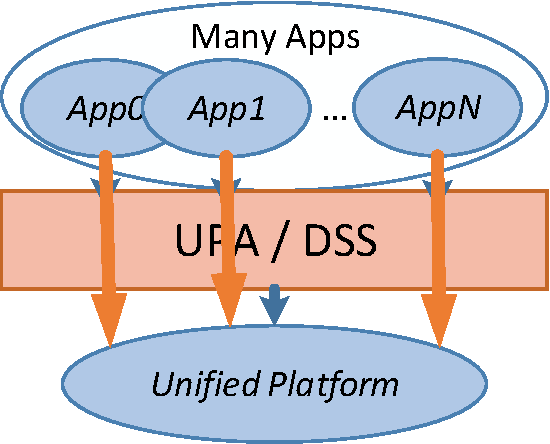
\includegraphics[width=.28\linewidth]{fig/DSSMAAR.pdf}\label{fig:mapMAAR}}
		\hfill
		\subfloat[FDP] {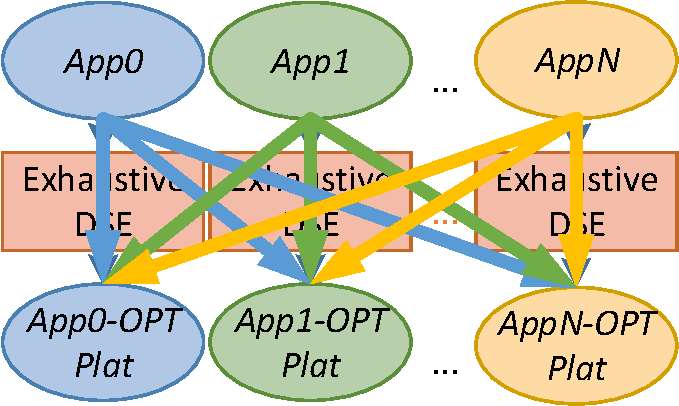
\includegraphics[width=.32\linewidth]{fig/FOP.pdf}\label{fig:mapFOP}}
		\hfill
		\subfloat[ODP] {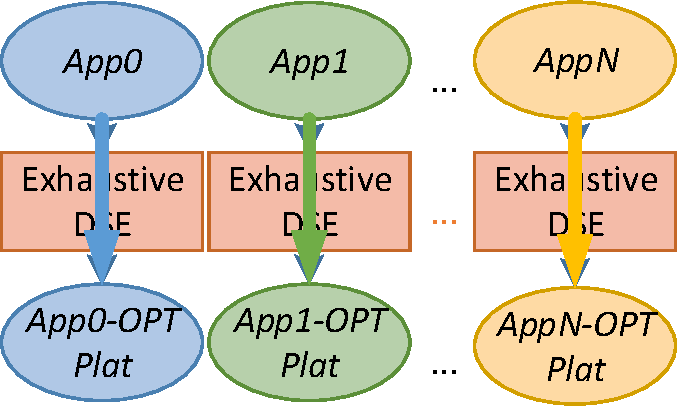
\includegraphics[width=.32\linewidth]{fig/OOP.pdf}\label{fig:mapOOP}}
	\vspace{-8pt}
	\caption{Experiments Settings}
	\label{fig:avg}
\end{figure}

\newtext{
To understand the benefits of UPA Evaluation, this section compares UPA with DSS~\cite{zhang2018ds} and Foreign Dedicated Platform (FDP). As \figref{fig:mapMAAR} shown, both UPA and DSS platform is designed for many applications. DSS is a greedy algorithm for platform allocation according to characteristics analysis across applications without an evaluation. While in \figref{fig:mapFOP}, FDP considers one application in isolation instead of many applications. In the experiments, an exhaustive search is used to find the dedicated platform, which gives the optimal platform for one application. Then mapping all applications on this platform provides one Foreign Dedicated Platform (FDP) performance. To get the average performance of FDP, this paper maps all applications onto all optimal platforms (one platform from one application). Similar to ODP, FDP results in the same number of platforms. However, ODP in \figref{fig:mapOOP} only maps the application on its Own Dedicated Platform (ODP), while FDP maps all applications onto each platform.
}

\newtext{
\begingroup
\setlength{\columnsep}{8pt}%
\begin{wrapfigure}{l}{0.5\linewidth}
	\vspace{-4pt}
	\begin{center}
		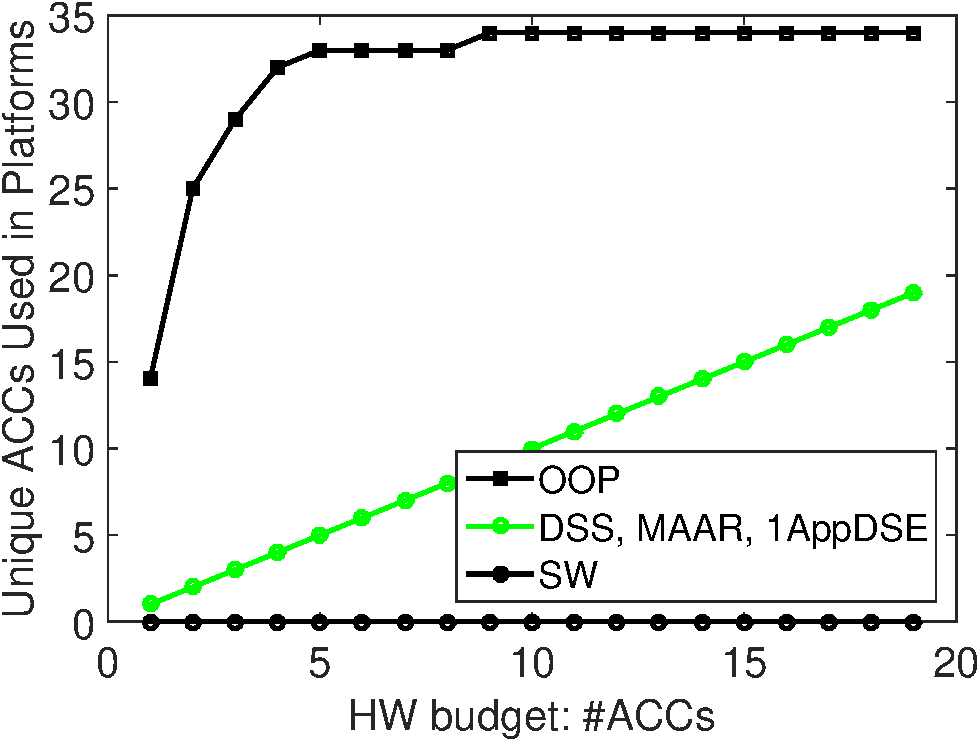
\includegraphics[width=\linewidth]{fig/oopHW.pdf}
	\end{center}
	\vspace{-8pt}
	\caption{Unique ACCs Used in Platform(s)}
	\label{fig:oopHW}
	\vspace{-4pt}
\end{wrapfigure}


\figref{fig:oopHW} lists the number of unique ACCs in platform(s) for each allocation
(SW is empty; DSS, UPA and FDP are equal to the budget). ODP has one platform per application, so there are 40 platforms for all applications. Each dedicated platform has a number of ACCs equal to the budget, so there are a large number of unique ACCs for all dedicated platforms. When each dedicated platform has 1 ACC, there are 14 unique ACCs, indicating some reuse. However, if each dedicated platform has 2 ACCs, there are 25 unique ACCs (11 more) showing the limits of reuse. 

\endgroup
}

\vspace{-2pt}
\subsection{Unified Platform Evaluation in Allocation}
\label{subsec:res-overall}



\newtext{
This section first analyzes the efficiency improvement in Section \ref{subsubsec:overall-sw}, and the efficiency achievement in Section \ref{subsubsec:overall-oop} for different allocations (DSS, UPA, and FDP). 
Section \ref{subsubsec:overall-time} compares their exploration time.
Finally, \secref{subsubsec:overall-acc} shows the detail of ACCs selection in a UPA platform. 
}
\subsubsection{Efficiency Improvement}
\label{subsubsec:overall-sw}

\begin{figure}[h]
\vspace{-8pt}
	\centering
		\subfloat[Average $rEFF_{SW}$] {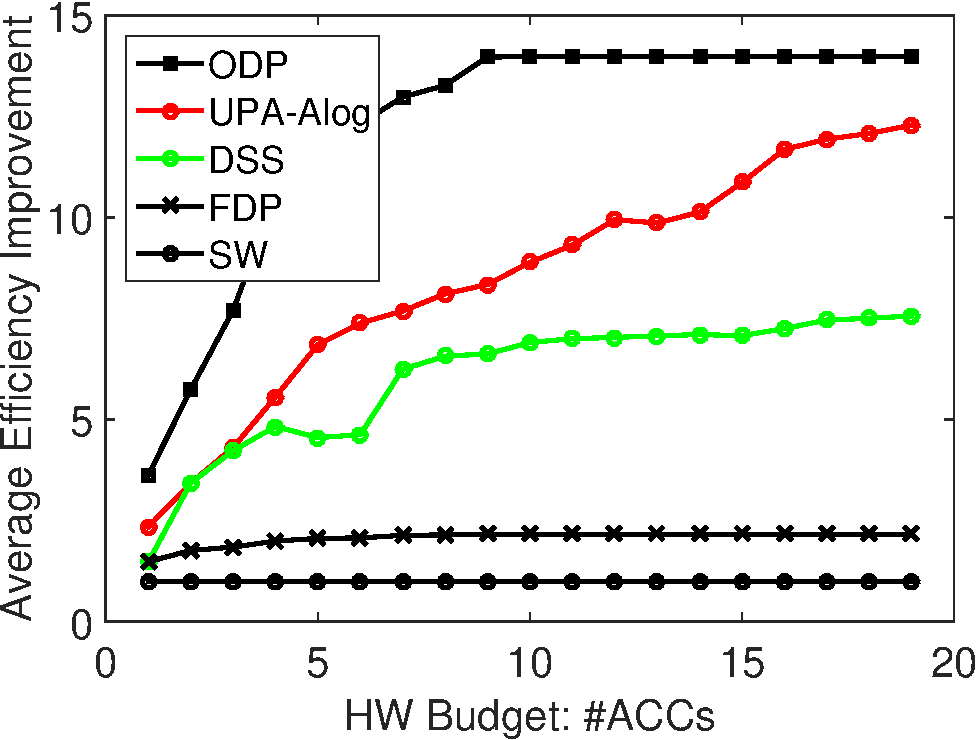
\includegraphics[width=.48\linewidth]{fig/allsw.pdf}\label{fig:allsw}}
		\hfill
		\subfloat[Cumulative Probability (ACCs=12)] {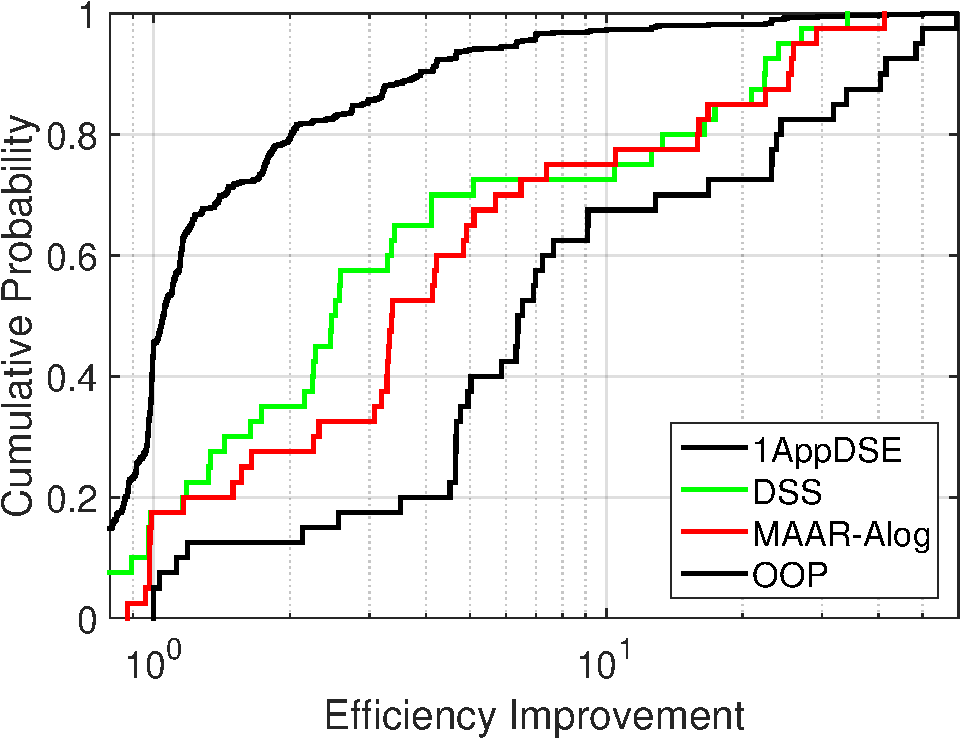
\includegraphics[width=.48\linewidth]{fig/MAARsw12all.pdf}\label{fig:sw12all}}
	\vspace{-8pt}
	\caption{Efficiency Improvement $rEFF_{SW}$}
	\label{fig:overallsw}
\end{figure}

\newtext{
\figref{fig:allsw} shows the average efficiency improvement ($rEEF_{SW}$) across all applications of different platform allocations over increasing ACCs budgets. ODP yields the absolute upper bound for a given HW constraints. ODP plateaus after ACCs=9, since each application only has up to 10 unique kernels. Since SW compared with itself, the $rEFF_{SW}$ value of SW is always equal to 1, which yields the lower bound. UPA uses $Alog$ (log area aggregation of $EEF$) evaluation. UPA-Alog's average efficiency improvement increases with the number of ACCs. It approaches the ODP efficiency when ACCs=19. With a 12 ACCs budget, UPA-Alog has 1.41 times the average efficiency improvement of DSS, and 4.59 times the improvement of FDP.
}

\newtext{
To give a detail comparison among different allocations, 
\figref{fig:sw12all} shows the cumulative probability of efficiency improvement for ODP, UPA, DSS and FDP with a ACCs=12 budget.} 
The x-axis denotes efficiency improvement ($rEFF_{SW}$), and y-axis is the cumulative probability.
A point ($x$, $y$) indicates that a proportion $y$ of applications have a relative efficiency $x$ or less.  
E.g. there is 67.5\% (0.675 in y-axis) probability that ODP has 10x ($10^1$ in x-axis) or 10x less efficiency improvement. In another description, ODP has 32.5\% ($1-0.675$ in y-axis) to achieve 10x or 10x more efficiency improvement. 

In \figref{fig:sw12all}, the line positioned more toward the bottom right has a better efficiency improvement, and ODP black line is the upper bound. 
\newtext{
SW can be considered as the lower bound, which has constant 1 efficiency improvement (i.e. vertical line $x = 10^0$ if drawn). 
As \figref{fig:sw12all} shown, UPA-Alog (red line) improves efficiency more than FDP (up left black line) and DSS (green line) for almost all applications. 
67.5\% ($1-0.325$ in y-axis) of applications have at least a 3x improvements, while FDP and DSS only improve 15\% ($1-0.85$) and 42.5\% ($1-0.575$) of applications respectively by the same amount. 
Note that FDP has a more smooth line, and shows more detail as it considers running any application on any application's dedicated optimal platform. 
}
\subsubsection{Efficiency Achievement View}
\label{subsubsec:overall-oop}

\begin{figure}[h]
\vspace{-8pt}
	\centering
		\subfloat[Average $rEFF_{OOP}$] {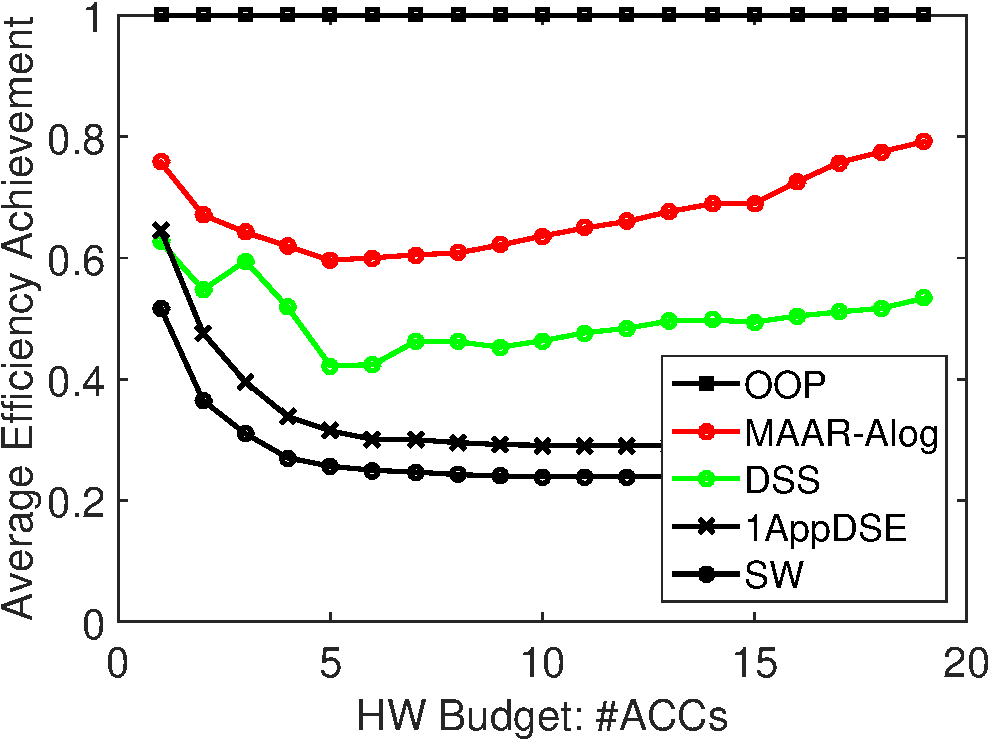
\includegraphics[width=.48\linewidth]{fig/alloop.pdf}\label{fig:alloop}}
		\hfill
		\subfloat[Cumulative Probability (ACCs=12)] {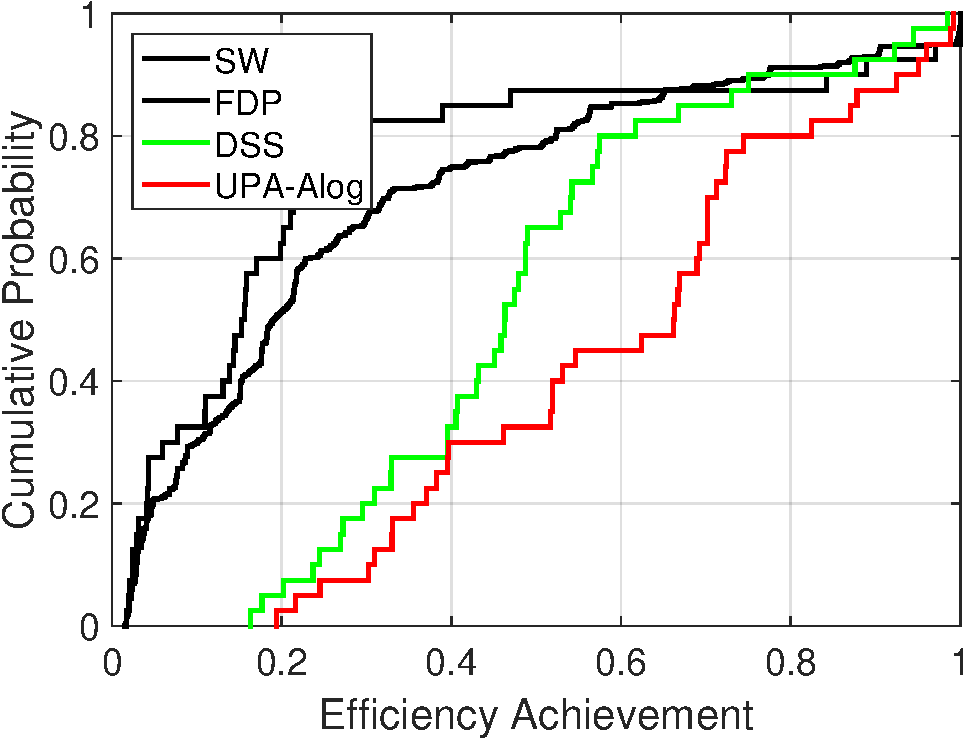
\includegraphics[width=.48\linewidth]{fig/MAARoop12all.pdf}\label{fig:oop12all}}
	\vspace{-8pt}
	\caption{Efficiency Achievement $rEFF_{OOP}$}
	\label{fig:overalloop}
\end{figure}

\figref{fig:alloop} shows the average efficiency achievement ($rEEF_{OOP}$) across all applications of different DSEs. 
\newtext{
OOP always achieves 100\% efficiency compared to itself (i.e. vertical line $x=1$ if drawn), and is the upper bound.}
SW has the lowest efficiency achievement, only reaching about 24\% after ACCs>9. 
\newtext{
MAAR DSE uses $Alog$ evaluation and produces a much better efficiency achievement than other DSEs.}
On average across the HW budgets, MAAR has 1.35 times the efficiency achievement of DSS, and 2.12 times the achievement of 1AppDSE.
\newtext{
\figref{fig:alloop} also shows that MAAR line is going down when ACCs<5, while it raises after ACCs>5.} It means that MAAR has a lower improvement speed than OOP when the HW budget is less than 5. However, after this point, MAAR improves faster than OOP. As OOP has already accelerated almost all computationally expensive kernels, there are less potential efficiency improvement for OOP.  

\newtext{
\figref{fig:oop12all} is the cumulative probability of efficiency achievement with 12 ACCs budget. Similar to \figref{fig:sw12all}, the line positioned more toward the bottom right has a better efficiency improvement, and MAAR has a significantly higher achievement than 1appDSE and DSS.
47.5\% ($1-0.525$ in y-axis) of applications obtain at least 60\% (in x-axis) efficiency of their dedicated OPT platform, while 1appDSE and DSS only has 12.5\% ($1-0.875$) and 10\% ($1-0.9$) of applications respectively achieving the same efficiency.
}

%Since efficiency achievement is relative to OOP, the plot of DSE can also describe the improvement speed between the DSE and OOP.
%MAAR is decreasing while ACCs<5, and increasing while ACCs>5. This 
\subsubsection{\newtext{Exploration Time}}
\label{subsubsec:overall-time}

\begin{figure}[h]
\vspace{-8pt}
	\centering
		\subfloat[OpenVX: Diff \#ACCs] {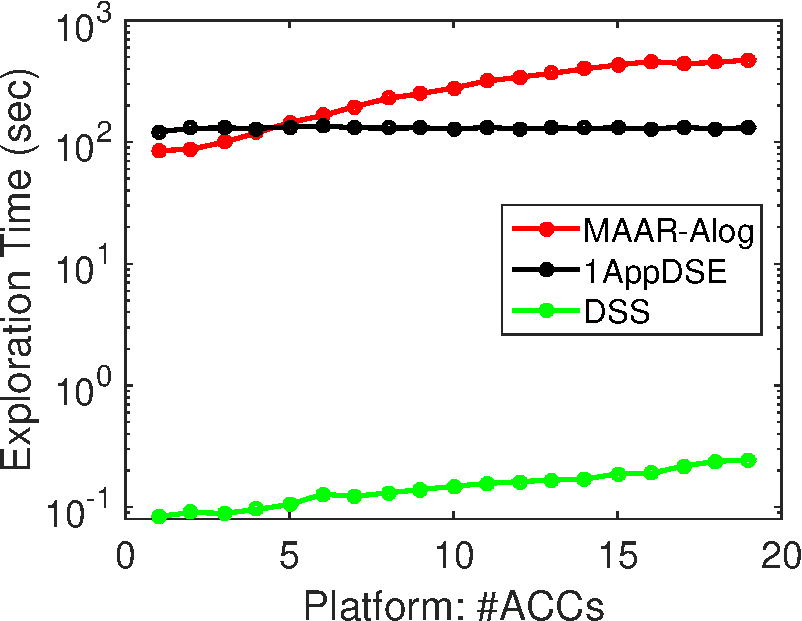
\includegraphics[width=.48\linewidth]{fig/timeACCs_all.pdf}\label{fig:timeACCs_all}}
		\hfill
		\subfloat[Synthetic: Diff \#Apps] {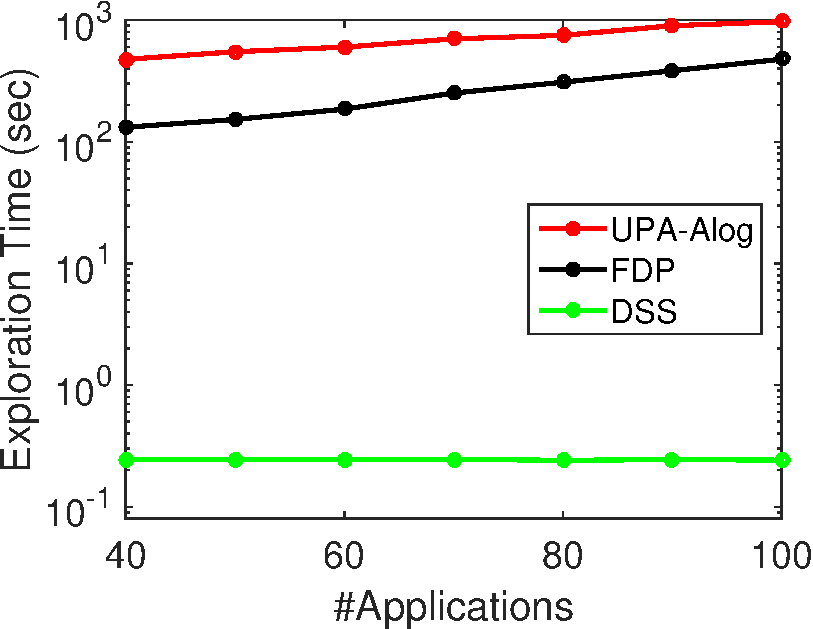
\includegraphics[width=.48\linewidth]{fig/timeApps_all.pdf}\label{fig:timeApps_all}}
	\vspace{-8pt}
	\caption{Exploration Time}
	\label{fig:exTime_all}
\end{figure}

\newtext{
\figref{fig:exTime_all} shows the exploration time of different allocations running on Intel i5-3450 with 3.10GHz.
\figref{fig:timeACCs_all} demonstrates the exploration time for OpenVX applications with an increasing ACC budget. Both DSS and UPA exploration time increases, because the platform design space gets bigger with the increasing number of ACCs. From ACCs=1 to ACCs=19, DSS's exploration time increases from 0.084 seconds to 0.245 seconds, and UPA is from 85.10 seconds to 475.56 seconds. DSS is much faster than UPA, since DSS is only a greedy selection algorithm and UPA contains a large number of evaluations. 
FDP has an almost constant exploration time because it is exhaustive search for each individual application, and the number of applications is fixed. With the number of ACCs increasing, the individual application design space does not increase much, because the number of unique kernels (ACC candidates) is only 2-9, while there are 35 kernels across many applications. 

\figref{fig:timeApps_all} shows the exploration time versus an increasing number of applications using synthetically generated applications. The total number of unique kernels in all application sets are 35, and the allocating platform(s) has a budget ACCs=19. 
The DSS exploration time is almost constant around 0.245 seconds, because it selects ACC using profiled characteristics from applications, and the number of applications does not impact on the exploration \cite{zhang2018ds}.
With increasing applications from 40 to 100, UPA exploration time increases from 475.56 seconds to 971.26 seconds, because it contains an increasing number of individual applications evaluation for each platform candidate.
Similarly, FDP exploration time increases significant from 131.65 seconds to 477.75 seconds, because of the more number of applications, the of more exhaustive search.   
}
\subsubsection{\newtext{UPA ACC Selection}}
\label{subsubsec:overall-acc}

\vspace{-2pt}

\begin{table}[h]
	\caption{Unified Platform Kernel Allocation}
	\label{tab:maar}
	\vspace{-8pt}
	\centering
	\begin{tabular}{|P{0.15\linewidth} | P{0.5\linewidth} | P{0.15\linewidth}|}
		\toprule
		\#ACCs & ACC Kernel Added & \#Used \\
		\midrule
		\hline
		1 & Custom Convolution & 37 \\
		\hline
		2 & Canny Edge Detector & 9 \\
		\hline
		3 & Harris Corners & 7 \\
		\hline
        4 & Optical Flow Pyramid (LK) & 4 \\
        \hline
        5 & Box Filter & 7 \\
        \hline
        6 & Gaussian Filter & 9\\
		\bottomrule
	\end{tabular}
\end{table}

\vspace{-2pt}



\tabref{tab:maar} shows UPA benefits when designing one unified platform for the OpenVX market with 1 to 6 ACCs. 
%gives insight on which OpenVX kernels MAAR chooses for a platform with 1 to 6 ACCs, as well as how often each ACC is used. 
All kernels are compute intense yielding a high efficiency improvement if accelerated. \textit{Custom Convolution} is most frequently used (39 times) as it is the basis of many vision kernels. For a platform with 2 ACCs, UPA adds \textit{Canny Edge} (9 times used). Overall, kernels appearing more frequently are not necessarily selected by UPA. Sometimes, less frequent but compute-intensive functions, e.g. \textit{Optical Flow Pyramid (LK)} added as a 4th ACC, have a higher priority.
However, this also indicates some limits of the input data flow graphs which were derived from the application's OpenVX calls. This kernel could be decomposed in many smaller kernels, which then subsequently could be reused more. 
Considering the specialization of kernels, e.g. \textit{Gaussian Filter} is a specialization of \textit{Convolution} which takes advantage of weight symmetries, is part of the future work.

\newtext{
This section demonstrates the limits of composability of dedicated platform allocation for single application. In \figref{fig:alloop}, the UPA with a 2 ACCs budget allocates \emph{Custom Convlution} and \emph{Canny Edge Detector} kernels, and achieves 67\% the average energy efficiency of ODP, which uses 25 unique ACCs in ODP shown in \figref{fig:oopHW}. It means a unified platform accelerating a small number of high-computing kernels can achieve good energy efficiency across many applications.
}

% the order of kernel in OpenVX allocation. CustomConvolution CannyEdgeDetector HarrisCorners OpticalFlowPyramid(LK)  BoxFilter GaussianFilter


%MAAR DSE design run-time is very moderate thanks to the fast heuristic GA traversal and a fast evaluation. Exploring a common platform with ACCs=19 for the 40 OpenVX applications on a 3.10GHz Intel i5-3450 only takes 147.56s.

%The number of unique kernels considered and the ACCs budget impact exploration time the most. Overall, the design space contains: $\frac{\#Kernel!}{\#ACC! (\#Kernel - \#ACC)!}$ (assuming any to any connection between ACCs) configurations. 
%The exploration duration is correlated to design space size. With a larger size, more GA iterations are needed on average to find high-performing configurations.
%Some concrete examples: Increasing the ACC budget from 1 to 19 increases the OpenVX exploration time from 1.5s to 147seconds. Assuming a constant 19 ACC budget, but a varying application set (synthetically generated) changing from 30 to 100 unique kernels increases DSE time from 92s to 1351s.

%In addition, exploration time increases linearly with number of applications as each one must be evaluated individually. Application size by itself does not impact exploration time. Conversely, the number of unique kernels and kernel connection per application linearly impact the time for analytic evaluation, thus influence exploration time.





\vspace{-2pt}
\subsection{Evaluating Aggregation Alternatives}
\label{subsec:res-agg}


\newtext{
To compare evaluating aggregations, this section first uses the cumulative probability of efficiency improvement in Section \ref{subsubsec:agg-sw} and efficiency achievement in Section \ref{subsubsec:agg-oop} for UPA with different aggregations to show their fairness. Then, Exploration time is compared in Section \ref{subsubsec:agg-time} to analyze their scalability.   
}
\subsubsection{Efficiency Improvement}
\label{subsubsec:agg-sw}

\begin{figure*}[]
\vspace{-10pt}
	\centering
		\subfloat[\#ACCs=6]{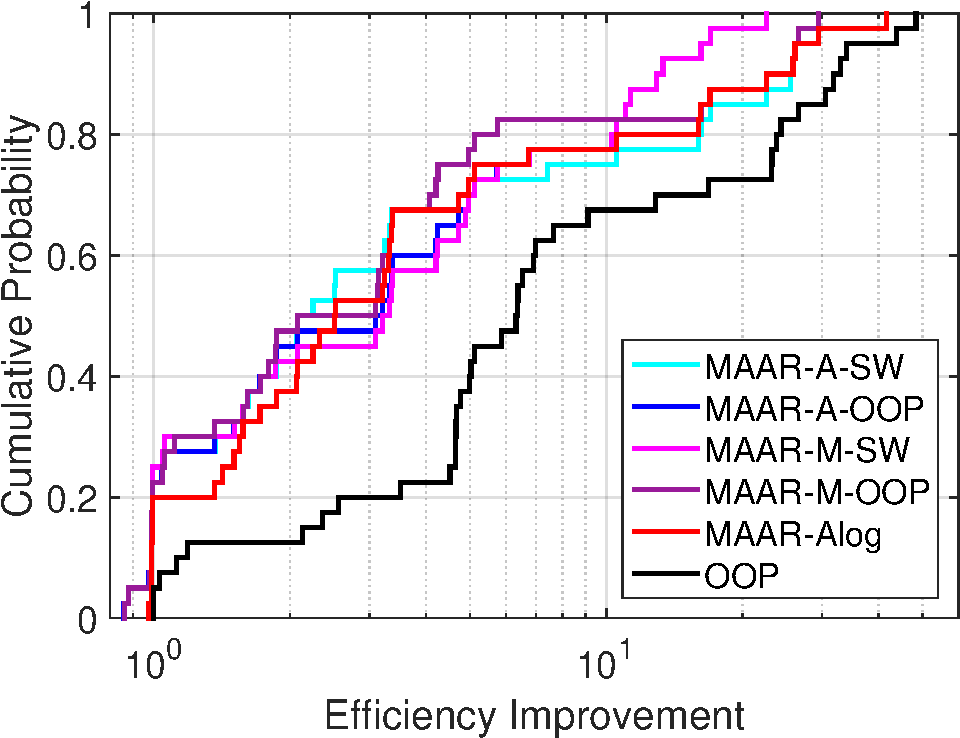
\includegraphics[width=.33\linewidth]{fig/MAARsw6.pdf}\label{fig:sw6}}
		\hfill
		\subfloat[\#ACCs=12]{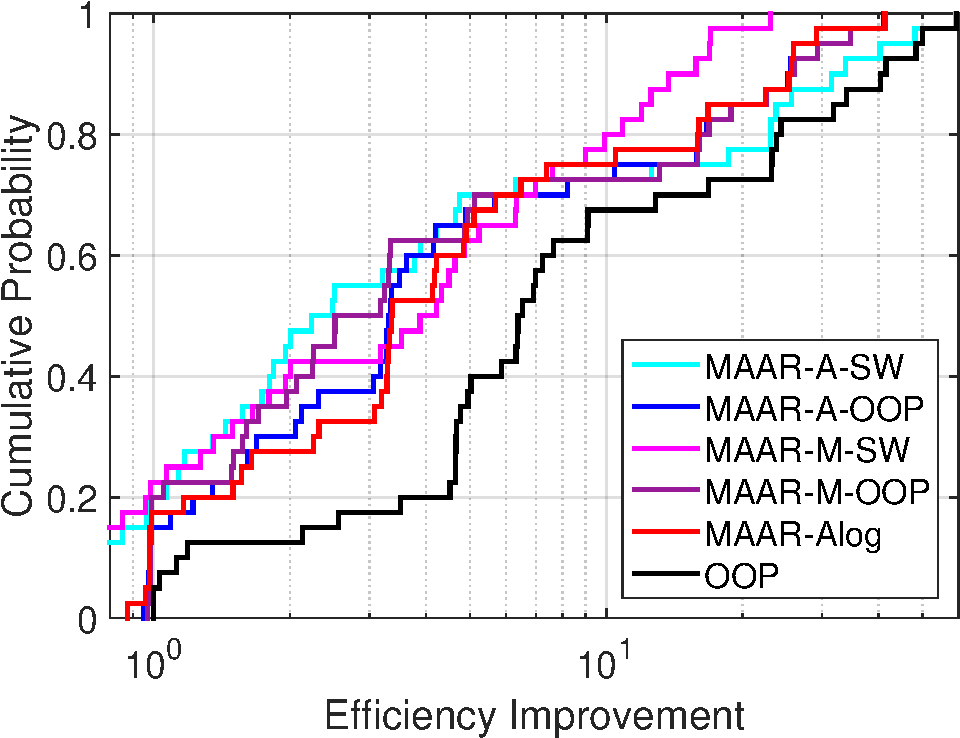
\includegraphics[width=.33\linewidth]{fig/MAARsw12.pdf}\label{fig:sw12}}
        \hfill
		\subfloat[\#ACCs=19]{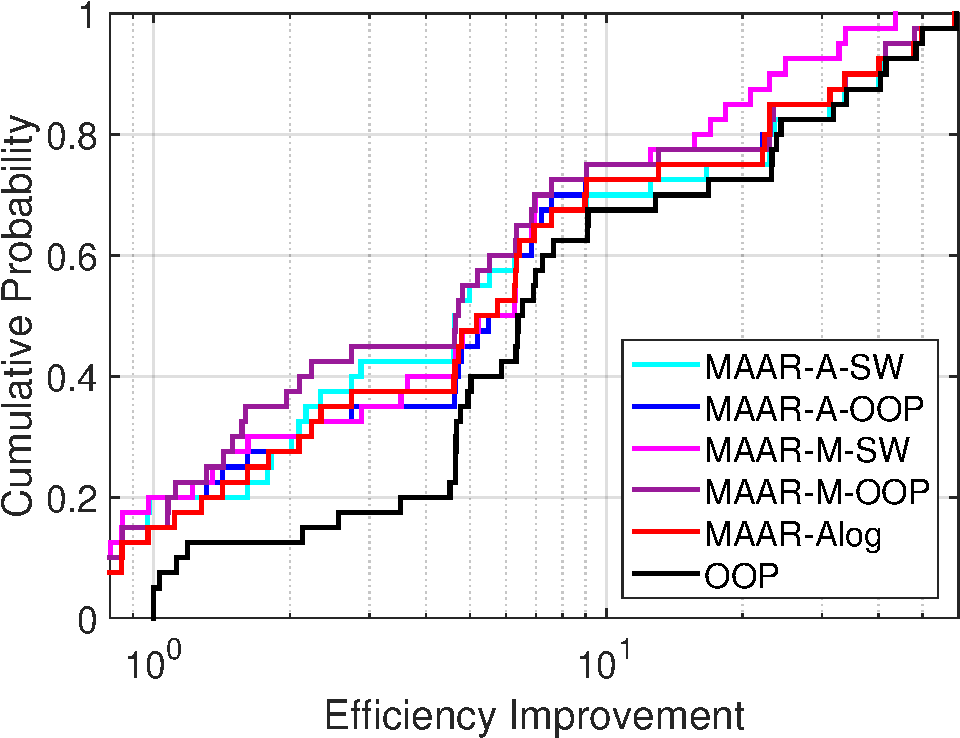
\includegraphics[width=.33\linewidth]{fig/MAARsw19.pdf}\label{fig:sw19}}
\vspace{-8pt}
	\caption{Relative Efficiency Compared with SW}
	\label{fig:OpenVXsw}
%		\vspace{-0pt}
\end{figure*}

%This section discusses the impact of aggregation on the fairness when allocating a common platform.
To visualize fairness, \figref{fig:OpenVXsw} shows the cumulative probability of efficiency improvement for ODP and UPA with different aggregations given a budget (ACCs = 6, 12, 19).
Similar to \figref{fig:sw12all}, the x-axis is efficiency improvement ($rEFF_{SW}$), and y-axis describes the cumulative probability. The line positioned more toward the bottom right has a better efficiency improvement, and OOP black line is the upper bound. 


%The x-axis denotes efficiency improvement ($rEFF_{SW}$), and y-axis is the cumulative probability.
%A point ($x$, $y$) indicates that a proportion $y$ of applications have a relative efficiency $x$ or less.  

%(so 1 - y\% have a relative efficiency of at least x).
%E.g., in \ref{fig:sw6}, there is 67.5\% (0.675 in y-axis) probability that OOP has 10x ($10^1$ in x-axis) or 10x less efficiency improvement. In another description, OOP has 32.5\% ($1-0.675$ in y-axis) to achieve 10x or 10x more efficiency improvement. The line positioned more toward the bottom right has a better efficiency improvement, and OOP black line is the upper bound.


With ACCs increasing from 6 (\figref{fig:sw6}) to 19 (\figref{fig:sw19}), the UPA lines move close to ODP line, which means the efficiency improvement of UPA platform are catching up to ODP performance. 
After ACCs>10, ODP has already allocated enough ACCs in each application-specific platform (mentioned in \figref{fig:allsw}), there are no remaining kernels to accelerate, then ODP lines are identical in \figref{fig:sw12} and \figref{fig:sw19}. 
In \figref{fig:OpenVXsw}, the up right parts of the lines represent high-efficiency applications, and the bottom left parts of lines show the effect of low-efficiency applications. 


%OOP lines are different between ACCs=6 and ACCs=12, but are identical between ACCs=12 and ACCs=19. The reason is that after ACCs>10, OOP has already allocated enough ACCs in each application-specific platform, and there are no remaining kernels to accelerate.


% The lines in these figures are similar to \figref{fig:effSW}, and represent efficiency improvement of each application. The difference between two types of figure is that \figref{fig:OpenVXsw} sorts the efficiency improvements for each DSE method independently and replace the applications with probability. As a result, each row in \figref{fig:effSW} represents the efficiency improvement of different methods for the same application, while \figref{fig:OpenVXsw} row may represent different applications. Then, 

Comparing among different UPA aggregation methods, 
$A\mhyphen SW$ is good for high-efficiency applications (top 25\%), however, has an efficiency loss for other applications, especially in \figref{fig:sw12}.
$A\mhyphen ODP$ has good efficiency improvement for all applications in all HW budgets.
$M\mhyphen SW$ only achieves good performance near the median-efficiency application, and there is a significant efficiency loss for all high-efficiency applications. 
$M\mhyphen ODP$ is bad in efficiency improvement view, and it loses in both median- and low-efficiency applications. 
$M\mhyphen SW$ and $M\mhyphen ODP$ shows the median $rEFF_{SW}$ and $rEFF_{ODP}$ aggregations of the same application set are actually different. 
$Alog$ achieves good efficiency improvement for all applications, with more focusing on low-efficiency applications, compared with another good evaluation $A\mhyphen ODP$.
\subsubsection{Efficiency Improvement View}
\label{subsubsec:agg-sw}

\begin{figure*}[]
\vspace{-10pt}
	\centering
		\subfloat[\#ACCs=6]{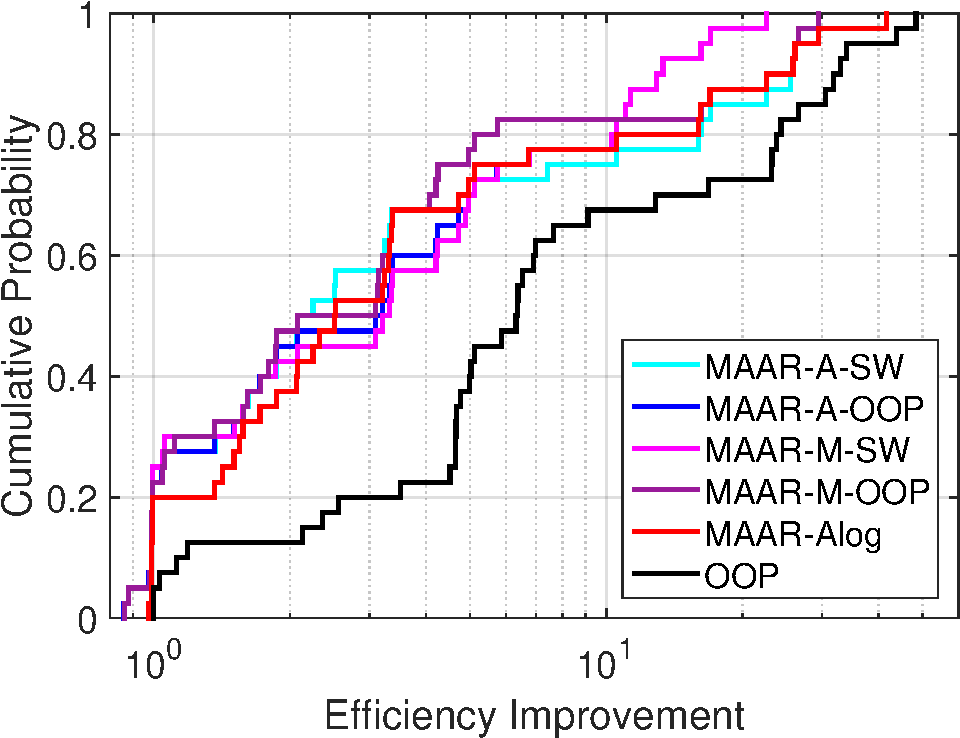
\includegraphics[width=.33\linewidth]{fig/MAARsw6.pdf}\label{fig:sw6}}
		\hfill
		\subfloat[\#ACCs=12]{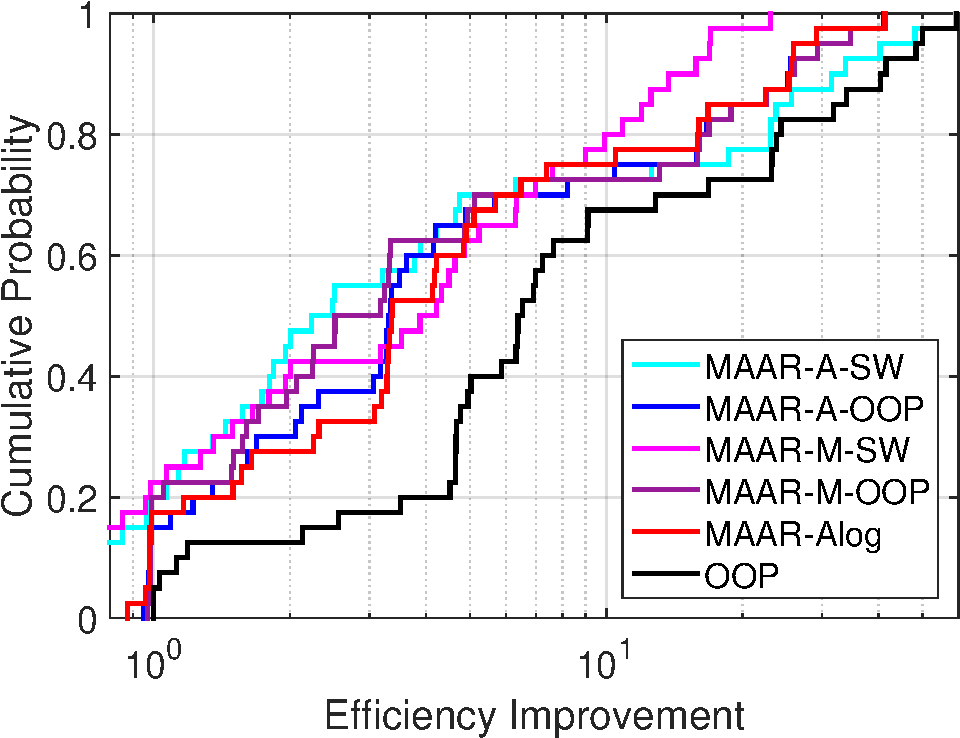
\includegraphics[width=.33\linewidth]{fig/MAARsw12.pdf}\label{fig:sw12}}
        \hfill
		\subfloat[\#ACCs=19]{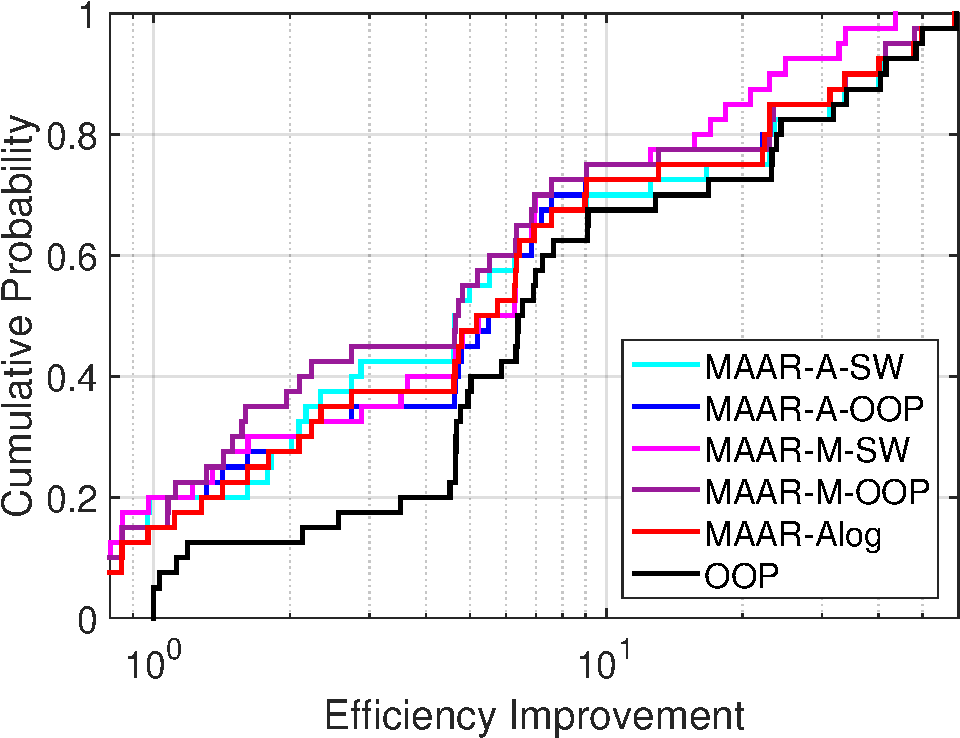
\includegraphics[width=.33\linewidth]{fig/MAARsw19.pdf}\label{fig:sw19}}
\vspace{-8pt}
	\caption{Relative Efficiency Compared with SW}
	\label{fig:OpenVXsw}
%		\vspace{-0pt}
\end{figure*}

%This section discusses the impact of aggregation on the fairness when allocating a common platform.
To visualize fairness, \figref{fig:OpenVXsw} shows the cumulative probability of efficiency improvement for OOP and MAAR DSE with different aggregations given a budget (ACCs = 6, 12, 19).
\newtext{
Similar to \figref{fig:sw12all}, the x-axis is efficiency improvement ($rEFF_{SW}$), and y-axis describes the cumulative probability. The line positioned more toward the bottom right has a better efficiency improvement, and OOP black line is the upper bound. 
}

%The x-axis denotes efficiency improvement ($rEFF_{SW}$), and y-axis is the cumulative probability.
%A point ($x$, $y$) indicates that a proportion $y$ of applications have a relative efficiency $x$ or less.  

%(so 1 - y\% have a relative efficiency of at least x).
%E.g., in \ref{fig:sw6}, there is 67.5\% (0.675 in y-axis) probability that OOP has 10x ($10^1$ in x-axis) or 10x less efficiency improvement. In another description, OOP has 32.5\% ($1-0.675$ in y-axis) to achieve 10x or 10x more efficiency improvement. The line positioned more toward the bottom right has a better efficiency improvement, and OOP black line is the upper bound.


With ACCs increasing from 6 (\figref{fig:sw6}) to 19 (\figref{fig:sw19}), the MAAR line moves close to OOP line, which means the efficiency improvement of MAAR platform are catching up to OOP performance. After ACCs>10, OOP has already allocated enough ACCs in each application-specific platform, \newtext{there are no remaining kernels to accelerate, then OOP lines are identical in \figref{fig:sw12} and \figref{fig:sw19}.} In \figref{fig:OpenVXsw}, the up right parts of the lines represent high-efficiency applications, and the bottom left parts of lines show the effect of low-efficiency applications. 


%OOP lines are different between ACCs=6 and ACCs=12, but are identical between ACCs=12 and ACCs=19. The reason is that after ACCs>10, OOP has already allocated enough ACCs in each application-specific platform, and there are no remaining kernels to accelerate.


% The lines in these figures are similar to \figref{fig:effSW}, and represent efficiency improvement of each application. The difference between two types of figure is that \figref{fig:OpenVXsw} sorts the efficiency improvements for each DSE method independently and replace the applications with probability. As a result, each row in \figref{fig:effSW} represents the efficiency improvement of different methods for the same application, while \figref{fig:OpenVXsw} row may represent different applications. Then, 

Comparing among different MAAR aggregation methods, 
$A\mhyphen SW$ is good for high-efficiency applications (top 25\%), however, has an efficiency loss for other applications, especially in \figref{fig:sw12}.
$A\mhyphen OOP$ has good efficiency improvement for all applications in all HW budgets.
$M\mhyphen SW$ only achieves good performance near the median-efficiency application, and there is a significant efficiency loss for all high-efficiency applications. 
$M\mhyphen OOP$ is bad in efficiency improvement view, and it loses in both median- and low-efficiency applications. 
$M\mhyphen SW$ and $M\mhyphen OOP$ shows the median $rEFF_{SW}$ and $rEFF_{OOP}$ aggregations of the same application set are actually different. 
$Alog$ achieves good efficiency improvement for all applications, with more focusing on low-efficiency applications, compared with another good evaluation $A\mhyphen OOP$.

\subsubsection{Exploration Time}
\label{subsubsec:agg-time}

\begin{figure}[h]
\vspace{-8pt}
	\centering
		\subfloat[OpenVX: Diff \#ACCs] {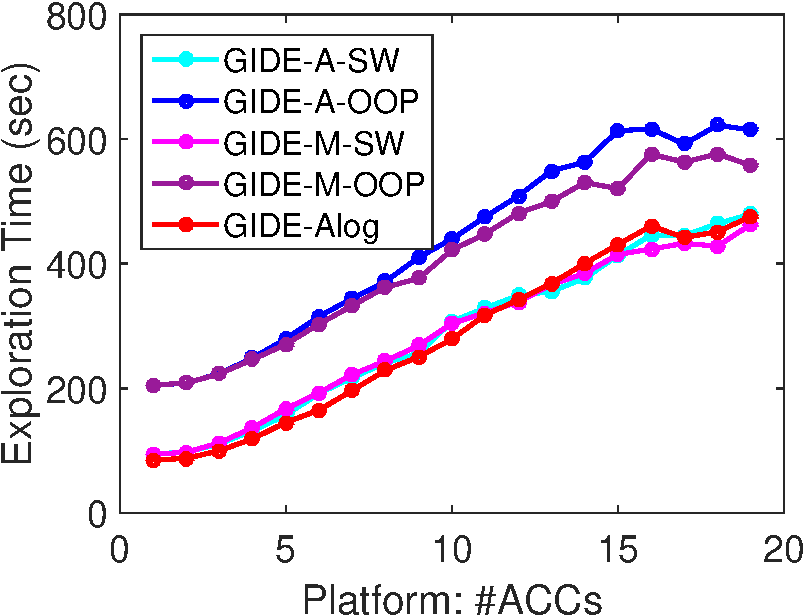
\includegraphics[width=.48\linewidth]{fig/timeACCs.pdf}\label{fig:timeACCs}}
		\hfill
		\subfloat[Synthetic: Diff \#Apps] {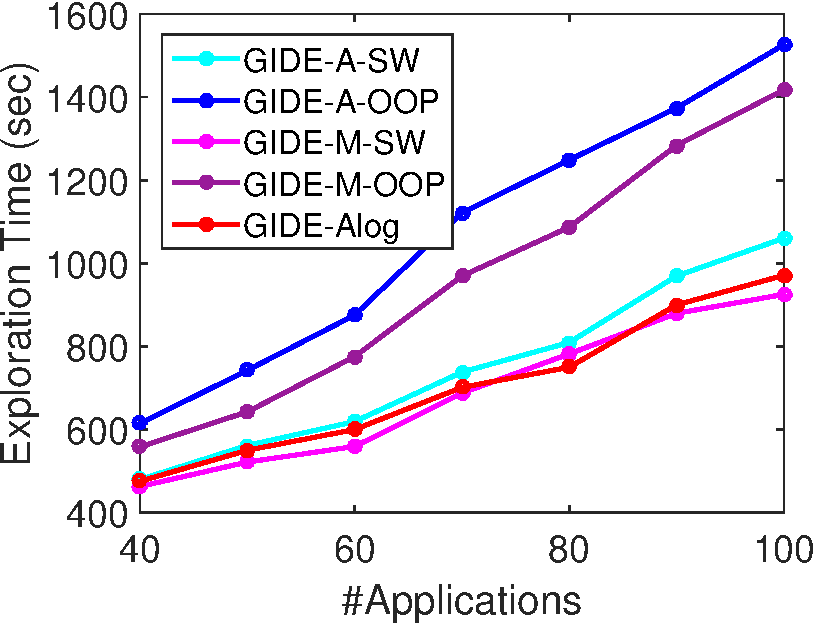
\includegraphics[width=.48\linewidth]{fig/timeApps.pdf}\label{fig:timeApps}}
	\vspace{-8pt}
	\caption{Exploration Time}
	\label{fig:exTime}
\end{figure}

\newtext{
\figref{fig:exTime} shows the exploration time  of MAAR DSE with different aggregations running on Intel i5-3450 with 3.10GHz. In \figref{fig:timeACCs}, the DSE exploration time increases with the increasing of ACCs budget.  
the $A \mhyphen OOP$ and $M \mhyphen OOP$ are much slower than other DSEs, because they need to find the OPT platform of each application for efficiency normalization. In average, the time of finding OPT platforms in $A \mhyphen OOP$ and $M \mhyphen OOP$ takes 32.56\% of total exploration. While, $A \mhyphen SW$, $M \mhyphen SW$ and $Alog$ evaluations do not need these OPT platforms. 
After ACCs>16, DSE exploration time stops increasing, because there is only 35 OpenVX unique kernels in applications, which could be instantiated once in HW. The design complexity of 16-19 ACCs from 35 kernels are not increased significantly.


\figref{fig:timeApps} describes the exploration time with increasing number of applications, which are synthetically generated.
With the number of application increasing, the $A \mhyphen OOP$ and $M \mhyphen OOP$ exploration time increases much faster than $A \mhyphen SW$, $M \mhyphen SW$ and $Alog$. The reason is that the number of application OPT platform search dramatic increases the exploration time of $M \mhyphen OOP$ and $A \mhyphen OOP$. 
}


\begin{table}[h]
	\caption{Comparison of Aggregations in MAAR DSE}
	\vspace{-8pt}
	\label{tab:cmp}
	\centering
	\begin{tabular}{p{0.125\linewidth}|p{0.25\linewidth}|p{0.25\linewidth}|p{0.175\linewidth}}
		\toprule
		& $rEFF_{SW}$ View & $rEFF_{OOP}$ View & Scalability \\
		\midrule
		
		\hline
		A-SW & Bad (low- med- EFF apps) & Bad (low- med- EFF apps) & Good \\
		\hline
		A-OOP & Good & Good & Bad \\
		\hline
		M-SW & Bad (high- EFF apps) & Bad (all apps) & Good \\
		\hline
		M-OOP & Bad (low- med- EFF apps) & Bad (low- EFF apps) & Bad \\
		\hline
		Alog & Good & Good & Good \\
		
		\bottomrule
	\end{tabular}
\end{table}

\newtext{
\tabref{tab:cmp} summaries the performance of MAAR DSE with different aggregations. $A \mhyphen SW$ has a good for scalability, however platform efficiency is bad for low- and med- efficiency applications. $A \mhyphen OOP$ platform achieves high efficient for all applications, but it has a bad scalability, since its normalization needs to explore the OPT platform for each application. Both $M \mhyphen SW$ and $M \mhyphen OOP$ platforms have bad efficiency, because they are only focus on the med- efficiency application in a certain view ($rEFF_{SW}$ or $rEFF_{OOP}$).
We select $Alog$ as aggregation, since it is efficient and fair to all applications. Moreover, it eliminates the need to compute the  normalization, i.e. finding the OPT platform for each application (a DSE problem in itself).
}

\vspace{-2pt}
\section{Conclusion}
\label{sec:conclusion}
This paper introduced a novel Design Space Exploration (DSE) approach for Many Applications Accelerator-Rich (MAAR) platforms. The aim of MAAR DSE is designing next generation of Accelerator-Rich platforms to address emerging computationally diverse markets such as computer vision and software-defined radio, by broadening the scope of DSE from a single application in isolation to many applications. The proposed MAAR DSE employs elitist GA for fast traversal and a fair evaluation methodology for balancing the focus and accelerator allocation across all applications. Our results on OpenVX applications demonstrate that MAAR DSE obtains 4.01 and 1.39 times more relative efficiency improvement than 1AppDSE and DSS respectively. With a 12 ACCs budget, MAAR platform supports more applications (67.5\%) with high efficiency (3x) which is much higher then existing solutions. 

%while 1AppDSE and DSS only support 15\% and 42.5\% applications respectively.

%We choose $Alog$ as the best, because it is most fair for low-efficiency applications, and it does not to need to normalize application efficiency.

%The MAAR-DSE proposed fair aggregation solutions to judge platform fitness qualitatively to balance efficiency and accelerator selection across all applications

\vspace{-0.5em}
%\bibliographystyle{ACM-Reference-Format}
\bibliographystyle{unsrt}
\bibliography{sigproc} 

\end{document}

